% Created by tikzDevice version 0.8.1 on 2015-07-23 17:51:32
% !TEX encoding = UTF-8 Unicode
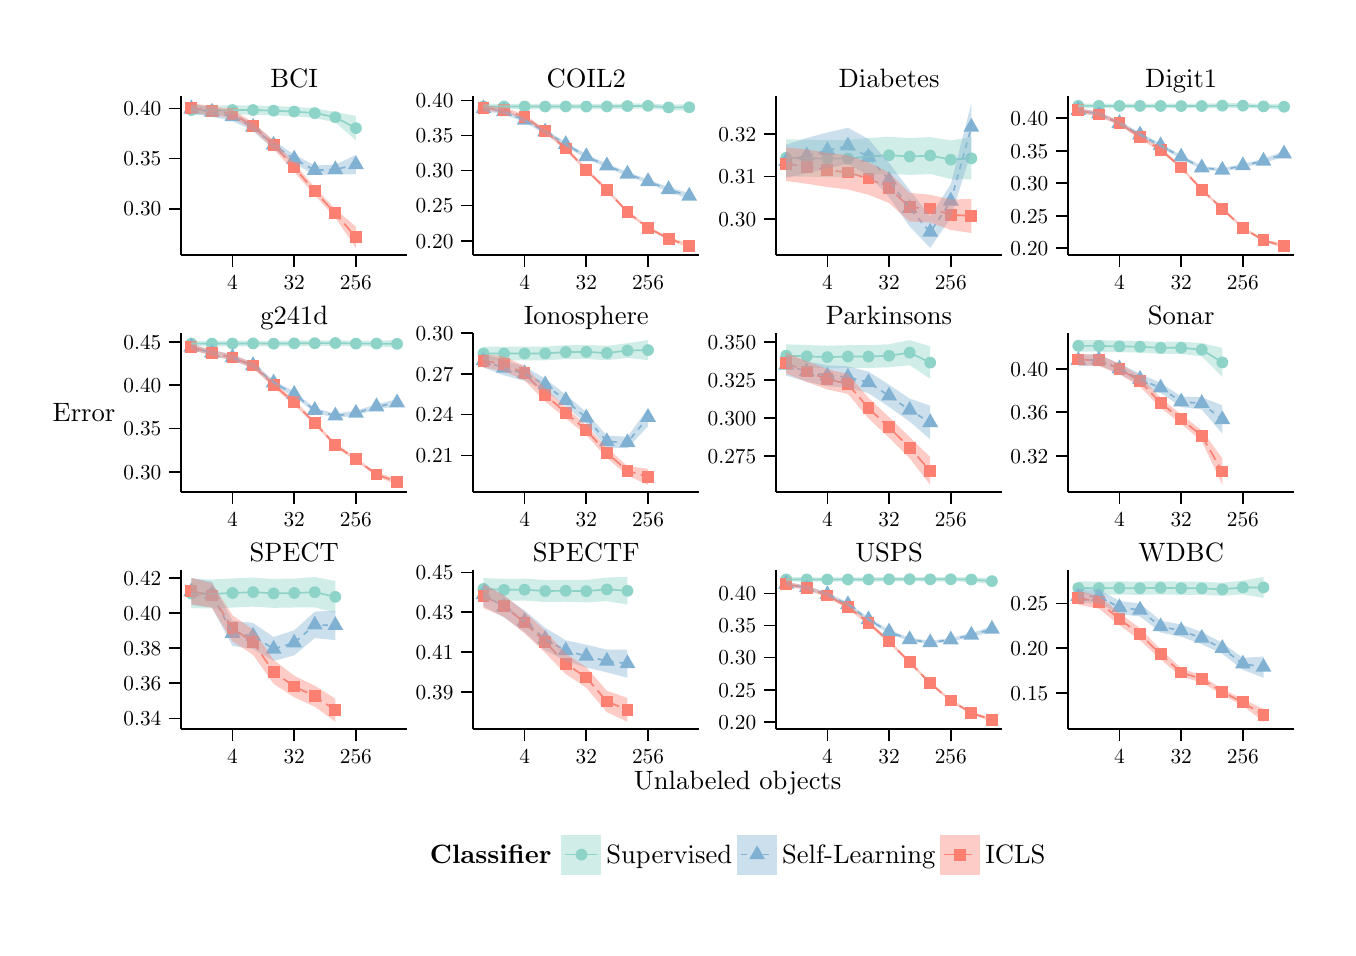
\begin{tikzpicture}[x=1pt,y=1pt]
\definecolor{fillColor}{RGB}{255,255,255}
\path[use as bounding box,fill=fillColor,fill opacity=0.00] (0,0) rectangle (469.75,325.21);
\begin{scope}
\path[clip] (  0.00,  0.00) rectangle (469.75,325.21);
\definecolor{drawColor}{RGB}{255,255,255}
\definecolor{fillColor}{RGB}{255,255,255}

\path[draw=drawColor,line width= 0.6pt,line join=round,line cap=round,fill=fillColor] (  0.00,  0.00) rectangle (469.75,325.21);
\end{scope}
\begin{scope}
\path[clip] ( 55.42,242.98) rectangle (137.20,300.54);
\definecolor{fillColor}{RGB}{255,255,255}

\path[fill=fillColor] ( 55.42,242.98) rectangle (137.20,300.54);
\definecolor{fillColor}{RGB}{141,211,199}

\path[fill=fillColor] ( 59.13,295.44) circle (  2.13);
\definecolor{fillColor}{RGB}{128,177,211}

\path[fill=fillColor] ( 59.13,299.26) --
	( 62.01,294.28) --
	( 56.26,294.28) --
	cycle;
\definecolor{fillColor}{RGB}{251,128,114}

\path[fill=fillColor] ( 57.00,294.12) --
	( 61.27,294.12) --
	( 61.27,298.38) --
	( 57.00,298.38) --
	cycle;
\definecolor{fillColor}{RGB}{141,211,199}

\path[fill=fillColor] ( 66.57,295.37) circle (  2.13);
\definecolor{fillColor}{RGB}{128,177,211}

\path[fill=fillColor] ( 66.57,298.05) --
	( 69.44,293.07) --
	( 63.69,293.07) --
	cycle;
\definecolor{fillColor}{RGB}{251,128,114}

\path[fill=fillColor] ( 64.43,293.04) --
	( 68.70,293.04) --
	( 68.70,297.31) --
	( 64.43,297.31) --
	cycle;
\definecolor{fillColor}{RGB}{141,211,199}

\path[fill=fillColor] ( 74.00,295.44) circle (  2.13);
\definecolor{fillColor}{RGB}{128,177,211}

\path[fill=fillColor] ( 74.00,296.42) --
	( 76.88,291.44) --
	( 71.13,291.44) --
	cycle;
\definecolor{fillColor}{RGB}{251,128,114}

\path[fill=fillColor] ( 71.87,291.99) --
	( 76.14,291.99) --
	( 76.14,296.26) --
	( 71.87,296.26) --
	cycle;
\definecolor{fillColor}{RGB}{141,211,199}

\path[fill=fillColor] ( 81.44,295.44) circle (  2.13);
\definecolor{fillColor}{RGB}{128,177,211}

\path[fill=fillColor] ( 81.44,292.61) --
	( 84.31,287.63) --
	( 78.56,287.63) --
	cycle;
\definecolor{fillColor}{RGB}{251,128,114}

\path[fill=fillColor] ( 79.30,287.49) --
	( 83.57,287.49) --
	( 83.57,291.76) --
	( 79.30,291.76) --
	cycle;
\definecolor{fillColor}{RGB}{141,211,199}

\path[fill=fillColor] ( 88.87,295.22) circle (  2.13);
\definecolor{fillColor}{RGB}{128,177,211}

\path[fill=fillColor] ( 88.87,286.12) --
	( 91.75,281.14) --
	( 86.00,281.14) --
	cycle;
\definecolor{fillColor}{RGB}{251,128,114}

\path[fill=fillColor] ( 86.74,280.80) --
	( 91.01,280.80) --
	( 91.01,285.07) --
	( 86.74,285.07) --
	cycle;
\definecolor{fillColor}{RGB}{141,211,199}

\path[fill=fillColor] ( 96.31,294.90) circle (  2.13);
\definecolor{fillColor}{RGB}{128,177,211}

\path[fill=fillColor] ( 96.31,281.10) --
	( 99.18,276.12) --
	( 93.43,276.12) --
	cycle;
\definecolor{fillColor}{RGB}{251,128,114}

\path[fill=fillColor] ( 94.17,272.56) --
	( 98.44,272.56) --
	( 98.44,276.83) --
	( 94.17,276.83) --
	cycle;
\definecolor{fillColor}{RGB}{141,211,199}

\path[fill=fillColor] (103.74,294.34) circle (  2.13);
\definecolor{fillColor}{RGB}{128,177,211}

\path[fill=fillColor] (103.74,277.01) --
	(106.62,272.03) --
	(100.87,272.03) --
	cycle;
\definecolor{fillColor}{RGB}{251,128,114}

\path[fill=fillColor] (101.61,263.94) --
	(105.88,263.94) --
	(105.88,268.21) --
	(101.61,268.21) --
	cycle;
\definecolor{fillColor}{RGB}{141,211,199}

\path[fill=fillColor] (111.18,292.85) circle (  2.13);
\definecolor{fillColor}{RGB}{128,177,211}

\path[fill=fillColor] (111.18,277.25) --
	(114.05,272.27) --
	(108.30,272.27) --
	cycle;
\definecolor{fillColor}{RGB}{251,128,114}

\path[fill=fillColor] (109.04,255.98) --
	(113.31,255.98) --
	(113.31,260.25) --
	(109.04,260.25) --
	cycle;
\definecolor{fillColor}{RGB}{141,211,199}

\path[fill=fillColor] (118.61,288.90) circle (  2.13);
\definecolor{fillColor}{RGB}{128,177,211}

\path[fill=fillColor] (118.61,279.07) --
	(121.49,274.09) --
	(115.74,274.09) --
	cycle;
\definecolor{fillColor}{RGB}{251,128,114}

\path[fill=fillColor] (116.48,247.32) --
	(120.75,247.32) --
	(120.75,251.58) --
	(116.48,251.58) --
	cycle;
\definecolor{drawColor}{RGB}{141,211,199}

\path[draw=drawColor,line width= 0.6pt,line join=round] ( 59.13,295.44) --
	( 66.57,295.37) --
	( 74.00,295.44) --
	( 81.44,295.44) --
	( 88.87,295.22) --
	( 96.31,294.90) --
	(103.74,294.34) --
	(111.18,292.85) --
	(118.61,288.90);
\definecolor{drawColor}{RGB}{128,177,211}

\path[draw=drawColor,line width= 0.6pt,dash pattern=on 2pt off 2pt ,line join=round] ( 59.13,295.94) --
	( 66.57,294.73) --
	( 74.00,293.10) --
	( 81.44,289.29) --
	( 88.87,282.80) --
	( 96.31,277.78) --
	(103.74,273.69) --
	(111.18,273.93) --
	(118.61,275.75);
\definecolor{drawColor}{RGB}{251,128,114}

\path[draw=drawColor,line width= 0.6pt,dash pattern=on 4pt off 2pt ,line join=round] ( 59.13,296.25) --
	( 66.57,295.18) --
	( 74.00,294.13) --
	( 81.44,289.63) --
	( 88.87,282.93) --
	( 96.31,274.69) --
	(103.74,266.07) --
	(111.18,258.12) --
	(118.61,249.45);
\definecolor{fillColor}{RGB}{141,211,199}

\path[fill=fillColor,fill opacity=0.40] ( 59.13,297.13) --
	( 66.57,297.06) --
	( 74.00,297.11) --
	( 81.44,297.11) --
	( 88.87,296.88) --
	( 96.31,296.63) --
	(103.74,296.09) --
	(111.18,294.75) --
	(118.61,293.30) --
	(118.61,284.49) --
	(111.18,290.95) --
	(103.74,292.59) --
	( 96.31,293.17) --
	( 88.87,293.55) --
	( 81.44,293.78) --
	( 74.00,293.76) --
	( 66.57,293.69) --
	( 59.13,293.75) --
	cycle;
\definecolor{fillColor}{RGB}{128,177,211}

\path[fill=fillColor,fill opacity=0.40] ( 59.13,297.58) --
	( 66.57,296.47) --
	( 74.00,294.67) --
	( 81.44,290.74) --
	( 88.87,284.37) --
	( 96.31,279.39) --
	(103.74,275.38) --
	(111.18,275.66) --
	(118.61,279.25) --
	(118.61,272.25) --
	(111.18,272.20) --
	(103.74,272.01) --
	( 96.31,276.17) --
	( 88.87,281.23) --
	( 81.44,287.84) --
	( 74.00,291.52) --
	( 66.57,293.00) --
	( 59.13,294.30) --
	cycle;
\definecolor{fillColor}{RGB}{251,128,114}

\path[fill=fillColor,fill opacity=0.40] ( 59.13,297.92) --
	( 66.57,296.88) --
	( 74.00,295.65) --
	( 81.44,290.92) --
	( 88.87,284.46) --
	( 96.31,276.33) --
	(103.74,267.47) --
	(111.18,259.67) --
	(118.61,253.30) --
	(118.61,245.60) --
	(111.18,256.56) --
	(103.74,264.68) --
	( 96.31,273.06) --
	( 88.87,281.40) --
	( 81.44,288.34) --
	( 74.00,292.61) --
	( 66.57,293.48) --
	( 59.13,294.58) --
	cycle;
\end{scope}
\begin{scope}
\path[clip] (160.97,242.98) rectangle (242.76,300.54);
\definecolor{fillColor}{RGB}{255,255,255}

\path[fill=fillColor] (160.97,242.98) rectangle (242.76,300.54);
\definecolor{fillColor}{RGB}{141,211,199}

\path[fill=fillColor] (164.69,296.71) circle (  2.13);
\definecolor{fillColor}{RGB}{128,177,211}

\path[fill=fillColor] (164.69,299.27) --
	(167.56,294.30) --
	(161.82,294.30) --
	cycle;
\definecolor{fillColor}{RGB}{251,128,114}

\path[fill=fillColor] (162.56,294.09) --
	(166.82,294.09) --
	(166.82,298.36) --
	(162.56,298.36) --
	cycle;
\definecolor{fillColor}{RGB}{141,211,199}

\path[fill=fillColor] (172.13,296.72) circle (  2.13);
\definecolor{fillColor}{RGB}{128,177,211}

\path[fill=fillColor] (172.13,298.25) --
	(175.00,293.27) --
	(169.25,293.27) --
	cycle;
\definecolor{fillColor}{RGB}{251,128,114}

\path[fill=fillColor] (169.99,293.33) --
	(174.26,293.33) --
	(174.26,297.60) --
	(169.99,297.60) --
	cycle;
\definecolor{fillColor}{RGB}{141,211,199}

\path[fill=fillColor] (179.56,296.73) circle (  2.13);
\definecolor{fillColor}{RGB}{128,177,211}

\path[fill=fillColor] (179.56,295.11) --
	(182.43,290.13) --
	(176.69,290.13) --
	cycle;
\definecolor{fillColor}{RGB}{251,128,114}

\path[fill=fillColor] (177.43,290.88) --
	(181.69,290.88) --
	(181.69,295.15) --
	(177.43,295.15) --
	cycle;
\definecolor{fillColor}{RGB}{141,211,199}

\path[fill=fillColor] (187.00,296.71) circle (  2.13);
\definecolor{fillColor}{RGB}{128,177,211}

\path[fill=fillColor] (187.00,290.93) --
	(189.87,285.95) --
	(184.12,285.95) --
	cycle;
\definecolor{fillColor}{RGB}{251,128,114}

\path[fill=fillColor] (184.86,285.62) --
	(189.13,285.62) --
	(189.13,289.89) --
	(184.86,289.89) --
	cycle;
\definecolor{fillColor}{RGB}{141,211,199}

\path[fill=fillColor] (194.43,296.74) circle (  2.13);
\definecolor{fillColor}{RGB}{128,177,211}

\path[fill=fillColor] (194.43,286.35) --
	(197.30,281.38) --
	(191.56,281.38) --
	cycle;
\definecolor{fillColor}{RGB}{251,128,114}

\path[fill=fillColor] (192.30,279.44) --
	(196.56,279.44) --
	(196.56,283.71) --
	(192.30,283.71) --
	cycle;
\definecolor{fillColor}{RGB}{141,211,199}

\path[fill=fillColor] (201.86,296.70) circle (  2.13);
\definecolor{fillColor}{RGB}{128,177,211}

\path[fill=fillColor] (201.86,282.00) --
	(204.74,277.02) --
	(198.99,277.02) --
	cycle;
\definecolor{fillColor}{RGB}{251,128,114}

\path[fill=fillColor] (199.73,271.70) --
	(204.00,271.70) --
	(204.00,275.97) --
	(199.73,275.97) --
	cycle;
\definecolor{fillColor}{RGB}{141,211,199}

\path[fill=fillColor] (209.30,296.74) circle (  2.13);
\definecolor{fillColor}{RGB}{128,177,211}

\path[fill=fillColor] (209.30,278.65) --
	(212.17,273.67) --
	(206.43,273.67) --
	cycle;
\definecolor{fillColor}{RGB}{251,128,114}

\path[fill=fillColor] (207.17,264.47) --
	(211.43,264.47) --
	(211.43,268.74) --
	(207.17,268.74) --
	cycle;
\definecolor{fillColor}{RGB}{141,211,199}

\path[fill=fillColor] (216.73,296.87) circle (  2.13);
\definecolor{fillColor}{RGB}{128,177,211}

\path[fill=fillColor] (216.73,275.68) --
	(219.61,270.70) --
	(213.86,270.70) --
	cycle;
\definecolor{fillColor}{RGB}{251,128,114}

\path[fill=fillColor] (214.60,256.41) --
	(218.87,256.41) --
	(218.87,260.68) --
	(214.60,260.68) --
	cycle;
\definecolor{fillColor}{RGB}{141,211,199}

\path[fill=fillColor] (224.17,296.96) circle (  2.13);
\definecolor{fillColor}{RGB}{128,177,211}

\path[fill=fillColor] (224.17,272.96) --
	(227.04,267.99) --
	(221.30,267.99) --
	cycle;
\definecolor{fillColor}{RGB}{251,128,114}

\path[fill=fillColor] (222.04,250.76) --
	(226.30,250.76) --
	(226.30,255.02) --
	(222.04,255.02) --
	cycle;
\definecolor{fillColor}{RGB}{141,211,199}

\path[fill=fillColor] (231.60,296.39) circle (  2.13);
\definecolor{fillColor}{RGB}{128,177,211}

\path[fill=fillColor] (231.60,270.07) --
	(234.48,265.09) --
	(228.73,265.09) --
	cycle;
\definecolor{fillColor}{RGB}{251,128,114}

\path[fill=fillColor] (229.47,246.84) --
	(233.74,246.84) --
	(233.74,251.11) --
	(229.47,251.11) --
	cycle;
\definecolor{fillColor}{RGB}{141,211,199}

\path[fill=fillColor] (239.04,296.44) circle (  2.13);
\definecolor{fillColor}{RGB}{128,177,211}

\path[fill=fillColor] (239.04,267.67) --
	(241.91,262.69) --
	(236.16,262.69) --
	cycle;
\definecolor{fillColor}{RGB}{251,128,114}

\path[fill=fillColor] (236.90,244.25) --
	(241.17,244.25) --
	(241.17,248.52) --
	(236.90,248.52) --
	cycle;
\definecolor{drawColor}{RGB}{141,211,199}

\path[draw=drawColor,line width= 0.6pt,line join=round] (164.69,296.71) --
	(172.13,296.72) --
	(179.56,296.73) --
	(187.00,296.71) --
	(194.43,296.74) --
	(201.86,296.70) --
	(209.30,296.74) --
	(216.73,296.87) --
	(224.17,296.96) --
	(231.60,296.39) --
	(239.04,296.44);
\definecolor{drawColor}{RGB}{128,177,211}

\path[draw=drawColor,line width= 0.6pt,dash pattern=on 2pt off 2pt ,line join=round] (164.69,295.96) --
	(172.13,294.93) --
	(179.56,291.79) --
	(187.00,287.61) --
	(194.43,283.04) --
	(201.86,278.68) --
	(209.30,275.33) --
	(216.73,272.36) --
	(224.17,269.65) --
	(231.60,266.75) --
	(239.04,264.35);
\definecolor{drawColor}{RGB}{251,128,114}

\path[draw=drawColor,line width= 0.6pt,dash pattern=on 4pt off 2pt ,line join=round] (164.69,296.22) --
	(172.13,295.46) --
	(179.56,293.02) --
	(187.00,287.75) --
	(194.43,281.57) --
	(201.86,273.84) --
	(209.30,266.61) --
	(216.73,258.54) --
	(224.17,252.89) --
	(231.60,248.97) --
	(239.04,246.39);
\definecolor{fillColor}{RGB}{141,211,199}

\path[fill=fillColor,fill opacity=0.40] (164.69,297.68) --
	(172.13,297.69) --
	(179.56,297.69) --
	(187.00,297.68) --
	(194.43,297.70) --
	(201.86,297.66) --
	(209.30,297.70) --
	(216.73,297.82) --
	(224.17,297.92) --
	(231.60,297.37) --
	(239.04,297.59) --
	(239.04,295.28) --
	(231.60,295.40) --
	(224.17,295.99) --
	(216.73,295.92) --
	(209.30,295.78) --
	(201.86,295.73) --
	(194.43,295.77) --
	(187.00,295.74) --
	(179.56,295.76) --
	(172.13,295.76) --
	(164.69,295.75) --
	cycle;
\definecolor{fillColor}{RGB}{128,177,211}

\path[fill=fillColor,fill opacity=0.40] (164.69,296.92) --
	(172.13,295.84) --
	(179.56,292.62) --
	(187.00,288.41) --
	(194.43,283.84) --
	(201.86,279.46) --
	(209.30,276.05) --
	(216.73,273.12) --
	(224.17,270.34) --
	(231.60,267.60) --
	(239.04,265.46) --
	(239.04,263.24) --
	(231.60,265.90) --
	(224.17,268.95) --
	(216.73,271.59) --
	(209.30,274.60) --
	(201.86,277.90) --
	(194.43,282.23) --
	(187.00,286.81) --
	(179.56,290.96) --
	(172.13,294.01) --
	(164.69,295.00) --
	cycle;
\definecolor{fillColor}{RGB}{251,128,114}

\path[fill=fillColor,fill opacity=0.40] (164.69,297.17) --
	(172.13,296.36) --
	(179.56,293.82) --
	(187.00,288.50) --
	(194.43,282.33) --
	(201.86,274.57) --
	(209.30,267.29) --
	(216.73,259.17) --
	(224.17,253.42) --
	(231.60,249.51) --
	(239.04,247.18) --
	(239.04,245.60) --
	(231.60,248.43) --
	(224.17,252.36) --
	(216.73,257.92) --
	(209.30,265.92) --
	(201.86,273.10) --
	(194.43,280.82) --
	(187.00,287.00) --
	(179.56,292.22) --
	(172.13,294.57) --
	(164.69,295.28) --
	cycle;
\end{scope}
\begin{scope}
\path[clip] (270.37,242.98) rectangle (352.15,300.54);
\definecolor{fillColor}{RGB}{255,255,255}

\path[fill=fillColor] (270.37,242.98) rectangle (352.15,300.54);
\definecolor{fillColor}{RGB}{141,211,199}

\path[fill=fillColor] (274.09,278.18) circle (  2.13);
\definecolor{fillColor}{RGB}{128,177,211}

\path[fill=fillColor] (274.09,280.23) --
	(276.96,275.25) --
	(271.21,275.25) --
	cycle;
\definecolor{fillColor}{RGB}{251,128,114}

\path[fill=fillColor] (271.95,273.73) --
	(276.22,273.73) --
	(276.22,278.00) --
	(271.95,278.00) --
	cycle;
\definecolor{fillColor}{RGB}{141,211,199}

\path[fill=fillColor] (281.52,278.05) circle (  2.13);
\definecolor{fillColor}{RGB}{128,177,211}

\path[fill=fillColor] (281.52,282.27) --
	(284.40,277.29) --
	(278.65,277.29) --
	cycle;
\definecolor{fillColor}{RGB}{251,128,114}

\path[fill=fillColor] (279.39,272.86) --
	(283.66,272.86) --
	(283.66,277.13) --
	(279.39,277.13) --
	cycle;
\definecolor{fillColor}{RGB}{141,211,199}

\path[fill=fillColor] (288.96,277.92) circle (  2.13);
\definecolor{fillColor}{RGB}{128,177,211}

\path[fill=fillColor] (288.96,284.18) --
	(291.83,279.20) --
	(286.08,279.20) --
	cycle;
\definecolor{fillColor}{RGB}{251,128,114}

\path[fill=fillColor] (286.82,271.66) --
	(291.09,271.66) --
	(291.09,275.93) --
	(286.82,275.93) --
	cycle;
\definecolor{fillColor}{RGB}{141,211,199}

\path[fill=fillColor] (296.39,277.91) circle (  2.13);
\definecolor{fillColor}{RGB}{128,177,211}

\path[fill=fillColor] (296.39,285.82) --
	(299.27,280.84) --
	(293.52,280.84) --
	cycle;
\definecolor{fillColor}{RGB}{251,128,114}

\path[fill=fillColor] (294.26,270.76) --
	(298.53,270.76) --
	(298.53,275.03) --
	(294.26,275.03) --
	cycle;
\definecolor{fillColor}{RGB}{141,211,199}

\path[fill=fillColor] (303.83,278.63) circle (  2.13);
\definecolor{fillColor}{RGB}{128,177,211}

\path[fill=fillColor] (303.83,281.78) --
	(306.70,276.81) --
	(300.95,276.81) --
	cycle;
\definecolor{fillColor}{RGB}{251,128,114}

\path[fill=fillColor] (301.69,268.56) --
	(305.96,268.56) --
	(305.96,272.83) --
	(301.69,272.83) --
	cycle;
\definecolor{fillColor}{RGB}{141,211,199}

\path[fill=fillColor] (311.26,279.13) circle (  2.13);
\definecolor{fillColor}{RGB}{128,177,211}

\path[fill=fillColor] (311.26,273.44) --
	(314.14,268.47) --
	(308.39,268.47) --
	cycle;
\definecolor{fillColor}{RGB}{251,128,114}

\path[fill=fillColor] (309.13,265.20) --
	(313.40,265.20) --
	(313.40,269.46) --
	(309.13,269.46) --
	cycle;
\definecolor{fillColor}{RGB}{141,211,199}

\path[fill=fillColor] (318.70,278.64) circle (  2.13);
\definecolor{fillColor}{RGB}{128,177,211}

\path[fill=fillColor] (318.70,263.24) --
	(321.57,258.26) --
	(315.82,258.26) --
	cycle;
\definecolor{fillColor}{RGB}{251,128,114}

\path[fill=fillColor] (316.56,258.19) --
	(320.83,258.19) --
	(320.83,262.46) --
	(316.56,262.46) --
	cycle;
\definecolor{fillColor}{RGB}{141,211,199}

\path[fill=fillColor] (326.13,278.99) circle (  2.13);
\definecolor{fillColor}{RGB}{128,177,211}

\path[fill=fillColor] (326.13,254.65) --
	(329.00,249.67) --
	(323.26,249.67) --
	cycle;
\definecolor{fillColor}{RGB}{251,128,114}

\path[fill=fillColor] (324.00,257.70) --
	(328.26,257.70) --
	(328.26,261.97) --
	(324.00,261.97) --
	cycle;
\definecolor{fillColor}{RGB}{141,211,199}

\path[fill=fillColor] (333.57,277.51) circle (  2.13);
\definecolor{fillColor}{RGB}{128,177,211}

\path[fill=fillColor] (333.57,265.91) --
	(336.44,260.94) --
	(330.69,260.94) --
	cycle;
\definecolor{fillColor}{RGB}{251,128,114}

\path[fill=fillColor] (331.43,255.49) --
	(335.70,255.49) --
	(335.70,259.76) --
	(331.43,259.76) --
	cycle;
\definecolor{fillColor}{RGB}{141,211,199}

\path[fill=fillColor] (341.00,277.99) circle (  2.13);
\definecolor{fillColor}{RGB}{128,177,211}

\path[fill=fillColor] (341.00,292.58) --
	(343.87,287.60) --
	(338.13,287.60) --
	cycle;
\definecolor{fillColor}{RGB}{251,128,114}

\path[fill=fillColor] (338.87,255.00) --
	(343.13,255.00) --
	(343.13,259.27) --
	(338.87,259.27) --
	cycle;
\definecolor{drawColor}{RGB}{141,211,199}

\path[draw=drawColor,line width= 0.6pt,line join=round] (274.09,278.18) --
	(281.52,278.05) --
	(288.96,277.92) --
	(296.39,277.91) --
	(303.83,278.63) --
	(311.26,279.13) --
	(318.70,278.64) --
	(326.13,278.99) --
	(333.57,277.51) --
	(341.00,277.99);
\definecolor{drawColor}{RGB}{128,177,211}

\path[draw=drawColor,line width= 0.6pt,dash pattern=on 2pt off 2pt ,line join=round] (274.09,276.91) --
	(281.52,278.95) --
	(288.96,280.86) --
	(296.39,282.50) --
	(303.83,278.46) --
	(311.26,270.13) --
	(318.70,259.92) --
	(326.13,251.33) --
	(333.57,262.60) --
	(341.00,289.26);
\definecolor{drawColor}{RGB}{251,128,114}

\path[draw=drawColor,line width= 0.6pt,dash pattern=on 4pt off 2pt ,line join=round] (274.09,275.87) --
	(281.52,274.99) --
	(288.96,273.79) --
	(296.39,272.89) --
	(303.83,270.70) --
	(311.26,267.33) --
	(318.70,260.32) --
	(326.13,259.84) --
	(333.57,257.63) --
	(341.00,257.14);
\definecolor{fillColor}{RGB}{141,211,199}

\path[fill=fillColor,fill opacity=0.40] (274.09,284.86) --
	(281.52,284.72) --
	(288.96,284.61) --
	(296.39,284.61) --
	(303.83,285.33) --
	(311.26,285.79) --
	(318.70,285.30) --
	(326.13,285.66) --
	(333.57,284.49) --
	(341.00,285.61) --
	(341.00,270.38) --
	(333.57,270.53) --
	(326.13,272.33) --
	(318.70,271.99) --
	(311.26,272.48) --
	(303.83,271.93) --
	(296.39,271.22) --
	(288.96,271.23) --
	(281.52,271.37) --
	(274.09,271.50) --
	cycle;
\definecolor{fillColor}{RGB}{128,177,211}

\path[fill=fillColor,fill opacity=0.40] (274.09,282.92) --
	(281.52,285.36) --
	(288.96,287.31) --
	(296.39,289.05) --
	(303.83,284.95) --
	(311.26,276.30) --
	(318.70,266.48) --
	(326.13,257.07) --
	(333.57,268.68) --
	(341.00,297.92) --
	(341.00,280.60) --
	(333.57,256.51) --
	(326.13,245.60) --
	(318.70,253.36) --
	(311.26,263.95) --
	(303.83,271.98) --
	(296.39,275.95) --
	(288.96,274.41) --
	(281.52,272.54) --
	(274.09,270.91) --
	cycle;
\definecolor{fillColor}{RGB}{251,128,114}

\path[fill=fillColor,fill opacity=0.40] (274.09,281.96) --
	(281.52,281.16) --
	(288.96,279.96) --
	(296.39,279.07) --
	(303.83,276.55) --
	(311.26,272.81) --
	(318.70,265.49) --
	(326.13,264.84) --
	(333.57,263.14) --
	(341.00,263.28) --
	(341.00,251.00) --
	(333.57,252.11) --
	(326.13,254.84) --
	(318.70,255.15) --
	(311.26,261.85) --
	(303.83,264.84) --
	(296.39,266.72) --
	(288.96,267.63) --
	(281.52,268.82) --
	(274.09,269.78) --
	cycle;
\end{scope}
\begin{scope}
\path[clip] (375.93,242.98) rectangle (457.71,300.54);
\definecolor{fillColor}{RGB}{255,255,255}

\path[fill=fillColor] (375.93,242.98) rectangle (457.71,300.54);
\definecolor{fillColor}{RGB}{141,211,199}

\path[fill=fillColor] (379.64,296.94) circle (  2.13);
\definecolor{fillColor}{RGB}{128,177,211}

\path[fill=fillColor] (379.64,298.65) --
	(382.52,293.67) --
	(376.77,293.67) --
	cycle;
\definecolor{fillColor}{RGB}{251,128,114}

\path[fill=fillColor] (377.51,293.25) --
	(381.78,293.25) --
	(381.78,297.52) --
	(377.51,297.52) --
	cycle;
\definecolor{fillColor}{RGB}{141,211,199}

\path[fill=fillColor] (387.08,296.93) circle (  2.13);
\definecolor{fillColor}{RGB}{128,177,211}

\path[fill=fillColor] (387.08,297.38) --
	(389.95,292.40) --
	(384.21,292.40) --
	cycle;
\definecolor{fillColor}{RGB}{251,128,114}

\path[fill=fillColor] (384.95,291.69) --
	(389.21,291.69) --
	(389.21,295.95) --
	(384.95,295.95) --
	cycle;
\definecolor{fillColor}{RGB}{141,211,199}

\path[fill=fillColor] (394.51,296.92) circle (  2.13);
\definecolor{fillColor}{RGB}{128,177,211}

\path[fill=fillColor] (394.51,293.99) --
	(397.39,289.01) --
	(391.64,289.01) --
	cycle;
\definecolor{fillColor}{RGB}{251,128,114}

\path[fill=fillColor] (392.38,288.61) --
	(396.65,288.61) --
	(396.65,292.88) --
	(392.38,292.88) --
	cycle;
\definecolor{fillColor}{RGB}{141,211,199}

\path[fill=fillColor] (401.95,296.92) circle (  2.13);
\definecolor{fillColor}{RGB}{128,177,211}

\path[fill=fillColor] (401.95,289.83) --
	(404.82,284.85) --
	(399.08,284.85) --
	cycle;
\definecolor{fillColor}{RGB}{251,128,114}

\path[fill=fillColor] (399.82,283.50) --
	(404.08,283.50) --
	(404.08,287.77) --
	(399.82,287.77) --
	cycle;
\definecolor{fillColor}{RGB}{141,211,199}

\path[fill=fillColor] (409.38,296.90) circle (  2.13);
\definecolor{fillColor}{RGB}{128,177,211}

\path[fill=fillColor] (409.38,285.91) --
	(412.26,280.94) --
	(406.51,280.94) --
	cycle;
\definecolor{fillColor}{RGB}{251,128,114}

\path[fill=fillColor] (407.25,279.00) --
	(411.52,279.00) --
	(411.52,283.27) --
	(407.25,283.27) --
	cycle;
\definecolor{fillColor}{RGB}{141,211,199}

\path[fill=fillColor] (416.82,296.88) circle (  2.13);
\definecolor{fillColor}{RGB}{128,177,211}

\path[fill=fillColor] (416.82,281.83) --
	(419.69,276.86) --
	(413.94,276.86) --
	cycle;
\definecolor{fillColor}{RGB}{251,128,114}

\path[fill=fillColor] (414.68,272.57) --
	(418.95,272.57) --
	(418.95,276.83) --
	(414.68,276.83) --
	cycle;
\definecolor{fillColor}{RGB}{141,211,199}

\path[fill=fillColor] (424.25,296.89) circle (  2.13);
\definecolor{fillColor}{RGB}{128,177,211}

\path[fill=fillColor] (424.25,277.92) --
	(427.13,272.94) --
	(421.38,272.94) --
	cycle;
\definecolor{fillColor}{RGB}{251,128,114}

\path[fill=fillColor] (422.12,264.52) --
	(426.39,264.52) --
	(426.39,268.79) --
	(422.12,268.79) --
	cycle;
\definecolor{fillColor}{RGB}{141,211,199}

\path[fill=fillColor] (431.69,297.03) circle (  2.13);
\definecolor{fillColor}{RGB}{128,177,211}

\path[fill=fillColor] (431.69,277.10) --
	(434.56,272.12) --
	(428.81,272.12) --
	cycle;
\definecolor{fillColor}{RGB}{251,128,114}

\path[fill=fillColor] (429.55,257.64) --
	(433.82,257.64) --
	(433.82,261.91) --
	(429.55,261.91) --
	cycle;
\definecolor{fillColor}{RGB}{141,211,199}

\path[fill=fillColor] (439.12,297.03) circle (  2.13);
\definecolor{fillColor}{RGB}{128,177,211}

\path[fill=fillColor] (439.12,278.67) --
	(442.00,273.70) --
	(436.25,273.70) --
	cycle;
\definecolor{fillColor}{RGB}{251,128,114}

\path[fill=fillColor] (436.99,250.71) --
	(441.26,250.71) --
	(441.26,254.97) --
	(436.99,254.97) --
	cycle;
\definecolor{fillColor}{RGB}{141,211,199}

\path[fill=fillColor] (446.56,296.76) circle (  2.13);
\definecolor{fillColor}{RGB}{128,177,211}

\path[fill=fillColor] (446.56,280.35) --
	(449.43,275.37) --
	(443.68,275.37) --
	cycle;
\definecolor{fillColor}{RGB}{251,128,114}

\path[fill=fillColor] (444.42,246.21) --
	(448.69,246.21) --
	(448.69,250.48) --
	(444.42,250.48) --
	cycle;
\definecolor{fillColor}{RGB}{141,211,199}

\path[fill=fillColor] (453.99,296.63) circle (  2.13);
\definecolor{fillColor}{RGB}{128,177,211}

\path[fill=fillColor] (453.99,282.93) --
	(456.87,277.95) --
	(451.12,277.95) --
	cycle;
\definecolor{fillColor}{RGB}{251,128,114}

\path[fill=fillColor] (451.86,244.15) --
	(456.13,244.15) --
	(456.13,248.42) --
	(451.86,248.42) --
	cycle;
\definecolor{drawColor}{RGB}{141,211,199}

\path[draw=drawColor,line width= 0.6pt,line join=round] (379.64,296.94) --
	(387.08,296.93) --
	(394.51,296.92) --
	(401.95,296.92) --
	(409.38,296.90) --
	(416.82,296.88) --
	(424.25,296.89) --
	(431.69,297.03) --
	(439.12,297.03) --
	(446.56,296.76) --
	(453.99,296.63);
\definecolor{drawColor}{RGB}{128,177,211}

\path[draw=drawColor,line width= 0.6pt,dash pattern=on 2pt off 2pt ,line join=round] (379.64,295.33) --
	(387.08,294.06) --
	(394.51,290.67) --
	(401.95,286.51) --
	(409.38,282.60) --
	(416.82,278.51) --
	(424.25,274.60) --
	(431.69,273.78) --
	(439.12,275.35) --
	(446.56,277.03) --
	(453.99,279.61);
\definecolor{drawColor}{RGB}{251,128,114}

\path[draw=drawColor,line width= 0.6pt,dash pattern=on 4pt off 2pt ,line join=round] (379.64,295.38) --
	(387.08,293.82) --
	(394.51,290.74) --
	(401.95,285.63) --
	(409.38,281.13) --
	(416.82,274.70) --
	(424.25,266.66) --
	(431.69,259.78) --
	(439.12,252.84) --
	(446.56,248.34) --
	(453.99,246.29);
\definecolor{fillColor}{RGB}{141,211,199}

\path[fill=fillColor,fill opacity=0.40] (379.64,297.79) --
	(387.08,297.78) --
	(394.51,297.77) --
	(401.95,297.76) --
	(409.38,297.74) --
	(416.82,297.73) --
	(424.25,297.75) --
	(431.69,297.91) --
	(439.12,297.92) --
	(446.56,297.65) --
	(453.99,297.70) --
	(453.99,295.56) --
	(446.56,295.88) --
	(439.12,296.15) --
	(431.69,296.16) --
	(424.25,296.04) --
	(416.82,296.02) --
	(409.38,296.05) --
	(401.95,296.07) --
	(394.51,296.08) --
	(387.08,296.09) --
	(379.64,296.10) --
	cycle;
\definecolor{fillColor}{RGB}{128,177,211}

\path[fill=fillColor,fill opacity=0.40] (379.64,296.12) --
	(387.08,294.85) --
	(394.51,291.40) --
	(401.95,287.32) --
	(409.38,283.31) --
	(416.82,279.22) --
	(424.25,275.21) --
	(431.69,274.43) --
	(439.12,276.04) --
	(446.56,277.81) --
	(453.99,280.64) --
	(453.99,278.58) --
	(446.56,276.25) --
	(439.12,274.67) --
	(431.69,273.14) --
	(424.25,273.99) --
	(416.82,277.81) --
	(409.38,281.89) --
	(401.95,285.70) --
	(394.51,289.94) --
	(387.08,293.28) --
	(379.64,294.54) --
	cycle;
\definecolor{fillColor}{RGB}{251,128,114}

\path[fill=fillColor,fill opacity=0.40] (379.64,296.18) --
	(387.08,294.63) --
	(394.51,291.51) --
	(401.95,286.41) --
	(409.38,281.86) --
	(416.82,275.29) --
	(424.25,267.23) --
	(431.69,260.37) --
	(439.12,253.39) --
	(446.56,248.86) --
	(453.99,246.98) --
	(453.99,245.60) --
	(446.56,247.82) --
	(439.12,252.29) --
	(431.69,259.18) --
	(424.25,266.09) --
	(416.82,274.10) --
	(409.38,280.40) --
	(401.95,284.86) --
	(394.51,289.98) --
	(387.08,293.01) --
	(379.64,294.59) --
	cycle;
\end{scope}
\begin{scope}
\path[clip] ( 55.42,157.38) rectangle (137.20,214.94);
\definecolor{fillColor}{RGB}{255,255,255}

\path[fill=fillColor] ( 55.42,157.38) rectangle (137.20,214.94);
\definecolor{fillColor}{RGB}{141,211,199}

\path[fill=fillColor] ( 59.13,211.05) circle (  2.13);
\definecolor{fillColor}{RGB}{128,177,211}

\path[fill=fillColor] ( 59.13,213.15) --
	( 62.01,208.18) --
	( 56.26,208.18) --
	cycle;
\definecolor{fillColor}{RGB}{251,128,114}

\path[fill=fillColor] ( 57.00,207.63) --
	( 61.27,207.63) --
	( 61.27,211.90) --
	( 57.00,211.90) --
	cycle;
\definecolor{fillColor}{RGB}{141,211,199}

\path[fill=fillColor] ( 66.57,211.05) circle (  2.13);
\definecolor{fillColor}{RGB}{128,177,211}

\path[fill=fillColor] ( 66.57,210.99) --
	( 69.44,206.01) --
	( 63.69,206.01) --
	cycle;
\definecolor{fillColor}{RGB}{251,128,114}

\path[fill=fillColor] ( 64.43,205.61) --
	( 68.70,205.61) --
	( 68.70,209.88) --
	( 64.43,209.88) --
	cycle;
\definecolor{fillColor}{RGB}{141,211,199}

\path[fill=fillColor] ( 74.00,211.07) circle (  2.13);
\definecolor{fillColor}{RGB}{128,177,211}

\path[fill=fillColor] ( 74.00,209.37) --
	( 76.88,204.39) --
	( 71.13,204.39) --
	cycle;
\definecolor{fillColor}{RGB}{251,128,114}

\path[fill=fillColor] ( 71.87,203.87) --
	( 76.14,203.87) --
	( 76.14,208.14) --
	( 71.87,208.14) --
	cycle;
\definecolor{fillColor}{RGB}{141,211,199}

\path[fill=fillColor] ( 81.44,211.11) circle (  2.13);
\definecolor{fillColor}{RGB}{128,177,211}

\path[fill=fillColor] ( 81.44,206.48) --
	( 84.31,201.50) --
	( 78.56,201.50) --
	cycle;
\definecolor{fillColor}{RGB}{251,128,114}

\path[fill=fillColor] ( 79.30,201.02) --
	( 83.57,201.02) --
	( 83.57,205.29) --
	( 79.30,205.29) --
	cycle;
\definecolor{fillColor}{RGB}{141,211,199}

\path[fill=fillColor] ( 88.87,211.02) circle (  2.13);
\definecolor{fillColor}{RGB}{128,177,211}

\path[fill=fillColor] ( 88.87,200.22) --
	( 91.75,195.24) --
	( 86.00,195.24) --
	cycle;
\definecolor{fillColor}{RGB}{251,128,114}

\path[fill=fillColor] ( 86.74,194.01) --
	( 91.01,194.01) --
	( 91.01,198.27) --
	( 86.74,198.27) --
	cycle;
\definecolor{fillColor}{RGB}{141,211,199}

\path[fill=fillColor] ( 96.31,211.14) circle (  2.13);
\definecolor{fillColor}{RGB}{128,177,211}

\path[fill=fillColor] ( 96.31,196.09) --
	( 99.18,191.11) --
	( 93.43,191.11) --
	cycle;
\definecolor{fillColor}{RGB}{251,128,114}

\path[fill=fillColor] ( 94.17,187.67) --
	( 98.44,187.67) --
	( 98.44,191.94) --
	( 94.17,191.94) --
	cycle;
\definecolor{fillColor}{RGB}{141,211,199}

\path[fill=fillColor] (103.74,211.19) circle (  2.13);
\definecolor{fillColor}{RGB}{128,177,211}

\path[fill=fillColor] (103.74,190.29) --
	(106.62,185.31) --
	(100.87,185.31) --
	cycle;
\definecolor{fillColor}{RGB}{251,128,114}

\path[fill=fillColor] (101.61,180.21) --
	(105.88,180.21) --
	(105.88,184.48) --
	(101.61,184.48) --
	cycle;
\definecolor{fillColor}{RGB}{141,211,199}

\path[fill=fillColor] (111.18,211.25) circle (  2.13);
\definecolor{fillColor}{RGB}{128,177,211}

\path[fill=fillColor] (111.18,188.28) --
	(114.05,183.30) --
	(108.30,183.30) --
	cycle;
\definecolor{fillColor}{RGB}{251,128,114}

\path[fill=fillColor] (109.04,172.27) --
	(113.31,172.27) --
	(113.31,176.54) --
	(109.04,176.54) --
	cycle;
\definecolor{fillColor}{RGB}{141,211,199}

\path[fill=fillColor] (118.61,211.05) circle (  2.13);
\definecolor{fillColor}{RGB}{128,177,211}

\path[fill=fillColor] (118.61,189.26) --
	(121.49,184.28) --
	(115.74,184.28) --
	cycle;
\definecolor{fillColor}{RGB}{251,128,114}

\path[fill=fillColor] (116.48,167.10) --
	(120.75,167.10) --
	(120.75,171.36) --
	(116.48,171.36) --
	cycle;
\definecolor{fillColor}{RGB}{141,211,199}

\path[fill=fillColor] (126.05,211.05) circle (  2.13);
\definecolor{fillColor}{RGB}{128,177,211}

\path[fill=fillColor] (126.05,191.58) --
	(128.92,186.60) --
	(123.17,186.60) --
	cycle;
\definecolor{fillColor}{RGB}{251,128,114}

\path[fill=fillColor] (123.91,161.62) --
	(128.18,161.62) --
	(128.18,165.89) --
	(123.91,165.89) --
	cycle;
\definecolor{fillColor}{RGB}{141,211,199}

\path[fill=fillColor] (133.48,210.95) circle (  2.13);
\definecolor{fillColor}{RGB}{128,177,211}

\path[fill=fillColor] (133.48,193.01) --
	(136.36,188.03) --
	(130.61,188.03) --
	cycle;
\definecolor{fillColor}{RGB}{251,128,114}

\path[fill=fillColor] (131.35,158.95) --
	(135.62,158.95) --
	(135.62,163.22) --
	(131.35,163.22) --
	cycle;
\definecolor{drawColor}{RGB}{141,211,199}

\path[draw=drawColor,line width= 0.6pt,line join=round] ( 59.13,211.05) --
	( 66.57,211.05) --
	( 74.00,211.07) --
	( 81.44,211.11) --
	( 88.87,211.02) --
	( 96.31,211.14) --
	(103.74,211.19) --
	(111.18,211.25) --
	(118.61,211.05) --
	(126.05,211.05) --
	(133.48,210.95);
\definecolor{drawColor}{RGB}{128,177,211}

\path[draw=drawColor,line width= 0.6pt,dash pattern=on 2pt off 2pt ,line join=round] ( 59.13,209.83) --
	( 66.57,207.67) --
	( 74.00,206.05) --
	( 81.44,203.16) --
	( 88.87,196.90) --
	( 96.31,192.77) --
	(103.74,186.97) --
	(111.18,184.96) --
	(118.61,185.94) --
	(126.05,188.26) --
	(133.48,189.69);
\definecolor{drawColor}{RGB}{251,128,114}

\path[draw=drawColor,line width= 0.6pt,dash pattern=on 4pt off 2pt ,line join=round] ( 59.13,209.77) --
	( 66.57,207.74) --
	( 74.00,206.00) --
	( 81.44,203.16) --
	( 88.87,196.14) --
	( 96.31,189.80) --
	(103.74,182.34) --
	(111.18,174.41) --
	(118.61,169.23) --
	(126.05,163.76) --
	(133.48,161.09);
\definecolor{fillColor}{RGB}{141,211,199}

\path[fill=fillColor,fill opacity=0.40] ( 59.13,212.05) --
	( 66.57,212.05) --
	( 74.00,212.07) --
	( 81.44,212.11) --
	( 88.87,212.03) --
	( 96.31,212.15) --
	(103.74,212.21) --
	(111.18,212.27) --
	(118.61,212.07) --
	(126.05,212.14) --
	(133.48,212.32) --
	(133.48,209.57) --
	(126.05,209.97) --
	(118.61,210.04) --
	(111.18,210.24) --
	(103.74,210.18) --
	( 96.31,210.12) --
	( 88.87,210.01) --
	( 81.44,210.10) --
	( 74.00,210.06) --
	( 66.57,210.06) --
	( 59.13,210.06) --
	cycle;
\definecolor{fillColor}{RGB}{128,177,211}

\path[fill=fillColor,fill opacity=0.40] ( 59.13,210.80) --
	( 66.57,208.71) --
	( 74.00,207.12) --
	( 81.44,204.18) --
	( 88.87,197.76) --
	( 96.31,193.71) --
	(103.74,187.81) --
	(111.18,185.81) --
	(118.61,186.81) --
	(126.05,189.16) --
	(133.48,190.99) --
	(133.48,188.39) --
	(126.05,187.36) --
	(118.61,185.06) --
	(111.18,184.11) --
	(103.74,186.13) --
	( 96.31,191.83) --
	( 88.87,196.04) --
	( 81.44,202.14) --
	( 74.00,204.99) --
	( 66.57,206.63) --
	( 59.13,208.87) --
	cycle;
\definecolor{fillColor}{RGB}{251,128,114}

\path[fill=fillColor,fill opacity=0.40] ( 59.13,210.74) --
	( 66.57,208.78) --
	( 74.00,207.06) --
	( 81.44,204.13) --
	( 88.87,197.03) --
	( 96.31,190.78) --
	(103.74,183.07) --
	(111.18,175.14) --
	(118.61,169.89) --
	(126.05,164.45) --
	(133.48,162.18) --
	(133.48,160.00) --
	(126.05,163.07) --
	(118.61,168.57) --
	(111.18,173.68) --
	(103.74,181.62) --
	( 96.31,188.83) --
	( 88.87,195.24) --
	( 81.44,202.18) --
	( 74.00,204.94) --
	( 66.57,206.71) --
	( 59.13,208.80) --
	cycle;
\end{scope}
\begin{scope}
\path[clip] (160.97,157.38) rectangle (242.76,214.94);
\definecolor{fillColor}{RGB}{255,255,255}

\path[fill=fillColor] (160.97,157.38) rectangle (242.76,214.94);
\definecolor{fillColor}{RGB}{141,211,199}

\path[fill=fillColor] (164.69,207.47) circle (  2.13);
\definecolor{fillColor}{RGB}{128,177,211}

\path[fill=fillColor] (164.69,208.22) --
	(167.56,203.24) --
	(161.82,203.24) --
	cycle;
\definecolor{fillColor}{RGB}{251,128,114}

\path[fill=fillColor] (162.56,202.69) --
	(166.82,202.69) --
	(166.82,206.95) --
	(162.56,206.95) --
	cycle;
\definecolor{fillColor}{RGB}{141,211,199}

\path[fill=fillColor] (172.13,207.46) circle (  2.13);
\definecolor{fillColor}{RGB}{128,177,211}

\path[fill=fillColor] (172.13,205.57) --
	(175.00,200.60) --
	(169.25,200.60) --
	cycle;
\definecolor{fillColor}{RGB}{251,128,114}

\path[fill=fillColor] (169.99,201.64) --
	(174.26,201.64) --
	(174.26,205.91) --
	(169.99,205.91) --
	cycle;
\definecolor{fillColor}{RGB}{141,211,199}

\path[fill=fillColor] (179.56,207.46) circle (  2.13);
\definecolor{fillColor}{RGB}{128,177,211}

\path[fill=fillColor] (179.56,203.53) --
	(182.43,198.55) --
	(176.69,198.55) --
	cycle;
\definecolor{fillColor}{RGB}{251,128,114}

\path[fill=fillColor] (177.43,198.21) --
	(181.69,198.21) --
	(181.69,202.47) --
	(177.43,202.47) --
	cycle;
\definecolor{fillColor}{RGB}{141,211,199}

\path[fill=fillColor] (187.00,207.51) circle (  2.13);
\definecolor{fillColor}{RGB}{128,177,211}

\path[fill=fillColor] (187.00,199.54) --
	(189.87,194.57) --
	(184.12,194.57) --
	cycle;
\definecolor{fillColor}{RGB}{251,128,114}

\path[fill=fillColor] (184.86,190.43) --
	(189.13,190.43) --
	(189.13,194.69) --
	(184.86,194.69) --
	cycle;
\definecolor{fillColor}{RGB}{141,211,199}

\path[fill=fillColor] (194.43,207.97) circle (  2.13);
\definecolor{fillColor}{RGB}{128,177,211}

\path[fill=fillColor] (194.43,193.85) --
	(197.30,188.87) --
	(191.56,188.87) --
	cycle;
\definecolor{fillColor}{RGB}{251,128,114}

\path[fill=fillColor] (192.30,183.91) --
	(196.56,183.91) --
	(196.56,188.17) --
	(192.30,188.17) --
	cycle;
\definecolor{fillColor}{RGB}{141,211,199}

\path[fill=fillColor] (201.86,208.05) circle (  2.13);
\definecolor{fillColor}{RGB}{128,177,211}

\path[fill=fillColor] (201.86,187.52) --
	(204.74,182.54) --
	(198.99,182.54) --
	cycle;
\definecolor{fillColor}{RGB}{251,128,114}

\path[fill=fillColor] (199.73,177.63) --
	(204.00,177.63) --
	(204.00,181.90) --
	(199.73,181.90) --
	cycle;
\definecolor{fillColor}{RGB}{141,211,199}

\path[fill=fillColor] (209.30,207.64) circle (  2.13);
\definecolor{fillColor}{RGB}{128,177,211}

\path[fill=fillColor] (209.30,178.97) --
	(212.17,173.99) --
	(206.43,173.99) --
	cycle;
\definecolor{fillColor}{RGB}{251,128,114}

\path[fill=fillColor] (207.17,169.42) --
	(211.43,169.42) --
	(211.43,173.69) --
	(207.17,173.69) --
	cycle;
\definecolor{fillColor}{RGB}{141,211,199}

\path[fill=fillColor] (216.73,208.53) circle (  2.13);
\definecolor{fillColor}{RGB}{128,177,211}

\path[fill=fillColor] (216.73,178.63) --
	(219.61,173.66) --
	(213.86,173.66) --
	cycle;
\definecolor{fillColor}{RGB}{251,128,114}

\path[fill=fillColor] (214.60,162.93) --
	(218.87,162.93) --
	(218.87,167.20) --
	(214.60,167.20) --
	cycle;
\definecolor{fillColor}{RGB}{141,211,199}

\path[fill=fillColor] (224.17,208.70) circle (  2.13);
\definecolor{fillColor}{RGB}{128,177,211}

\path[fill=fillColor] (224.17,187.74) --
	(227.04,182.77) --
	(221.30,182.77) --
	cycle;
\definecolor{fillColor}{RGB}{251,128,114}

\path[fill=fillColor] (222.04,160.78) --
	(226.30,160.78) --
	(226.30,165.05) --
	(222.04,165.05) --
	cycle;
\definecolor{drawColor}{RGB}{141,211,199}

\path[draw=drawColor,line width= 0.6pt,line join=round] (164.69,207.47) --
	(172.13,207.46) --
	(179.56,207.46) --
	(187.00,207.51) --
	(194.43,207.97) --
	(201.86,208.05) --
	(209.30,207.64) --
	(216.73,208.53) --
	(224.17,208.70);
\definecolor{drawColor}{RGB}{128,177,211}

\path[draw=drawColor,line width= 0.6pt,dash pattern=on 2pt off 2pt ,line join=round] (164.69,204.90) --
	(172.13,202.25) --
	(179.56,200.21) --
	(187.00,196.23) --
	(194.43,190.53) --
	(201.86,184.20) --
	(209.30,175.65) --
	(216.73,175.32) --
	(224.17,184.43);
\definecolor{drawColor}{RGB}{251,128,114}

\path[draw=drawColor,line width= 0.6pt,dash pattern=on 4pt off 2pt ,line join=round] (164.69,204.82) --
	(172.13,203.77) --
	(179.56,200.34) --
	(187.00,192.56) --
	(194.43,186.04) --
	(201.86,179.77) --
	(209.30,171.55) --
	(216.73,165.07) --
	(224.17,162.92);
\definecolor{fillColor}{RGB}{141,211,199}

\path[fill=fillColor,fill opacity=0.40] (164.69,209.96) --
	(172.13,209.96) --
	(179.56,209.96) --
	(187.00,210.00) --
	(194.43,210.49) --
	(201.86,210.59) --
	(209.30,210.23) --
	(216.73,211.18) --
	(224.17,212.32) --
	(224.17,205.08) --
	(216.73,205.89) --
	(209.30,205.06) --
	(201.86,205.51) --
	(194.43,205.46) --
	(187.00,205.02) --
	(179.56,204.97) --
	(172.13,204.97) --
	(164.69,204.98) --
	cycle;
\definecolor{fillColor}{RGB}{128,177,211}

\path[fill=fillColor,fill opacity=0.40] (164.69,207.35) --
	(172.13,204.94) --
	(179.56,202.83) --
	(187.00,198.37) --
	(194.43,192.66) --
	(201.86,186.27) --
	(209.30,177.76) --
	(216.73,177.39) --
	(224.17,187.66) --
	(224.17,181.19) --
	(216.73,173.24) --
	(209.30,173.53) --
	(201.86,182.13) --
	(194.43,188.41) --
	(187.00,194.08) --
	(179.56,197.60) --
	(172.13,199.57) --
	(164.69,202.45) --
	cycle;
\definecolor{fillColor}{RGB}{251,128,114}

\path[fill=fillColor,fill opacity=0.40] (164.69,207.25) --
	(172.13,206.46) --
	(179.56,202.96) --
	(187.00,194.98) --
	(194.43,188.07) --
	(201.86,181.56) --
	(209.30,173.39) --
	(216.73,166.76) --
	(224.17,165.83) --
	(224.17,160.00) --
	(216.73,163.37) --
	(209.30,169.72) --
	(201.86,177.98) --
	(194.43,184.01) --
	(187.00,190.14) --
	(179.56,197.72) --
	(172.13,201.09) --
	(164.69,202.39) --
	cycle;
\end{scope}
\begin{scope}
\path[clip] (270.37,157.38) rectangle (352.15,214.94);
\definecolor{fillColor}{RGB}{255,255,255}

\path[fill=fillColor] (270.37,157.38) rectangle (352.15,214.94);
\definecolor{fillColor}{RGB}{141,211,199}

\path[fill=fillColor] (274.09,206.69) circle (  2.13);
\definecolor{fillColor}{RGB}{128,177,211}

\path[fill=fillColor] (274.09,206.66) --
	(276.96,201.68) --
	(271.21,201.68) --
	cycle;
\definecolor{fillColor}{RGB}{251,128,114}

\path[fill=fillColor] (271.95,201.90) --
	(276.22,201.90) --
	(276.22,206.16) --
	(271.95,206.16) --
	cycle;
\definecolor{fillColor}{RGB}{141,211,199}

\path[fill=fillColor] (281.52,206.46) circle (  2.13);
\definecolor{fillColor}{RGB}{128,177,211}

\path[fill=fillColor] (281.52,204.27) --
	(284.40,199.29) --
	(278.65,199.29) --
	cycle;
\definecolor{fillColor}{RGB}{251,128,114}

\path[fill=fillColor] (279.39,198.82) --
	(283.66,198.82) --
	(283.66,203.08) --
	(279.39,203.08) --
	cycle;
\definecolor{fillColor}{RGB}{141,211,199}

\path[fill=fillColor] (288.96,206.16) circle (  2.13);
\definecolor{fillColor}{RGB}{128,177,211}

\path[fill=fillColor] (288.96,202.74) --
	(291.83,197.76) --
	(286.08,197.76) --
	cycle;
\definecolor{fillColor}{RGB}{251,128,114}

\path[fill=fillColor] (286.82,196.01) --
	(291.09,196.01) --
	(291.09,200.28) --
	(286.82,200.28) --
	cycle;
\definecolor{fillColor}{RGB}{141,211,199}

\path[fill=fillColor] (296.39,206.37) circle (  2.13);
\definecolor{fillColor}{RGB}{128,177,211}

\path[fill=fillColor] (296.39,202.30) --
	(299.27,197.32) --
	(293.52,197.32) --
	cycle;
\definecolor{fillColor}{RGB}{251,128,114}

\path[fill=fillColor] (294.26,194.34) --
	(298.53,194.34) --
	(298.53,198.61) --
	(294.26,198.61) --
	cycle;
\definecolor{fillColor}{RGB}{141,211,199}

\path[fill=fillColor] (303.83,206.35) circle (  2.13);
\definecolor{fillColor}{RGB}{128,177,211}

\path[fill=fillColor] (303.83,200.33) --
	(306.70,195.36) --
	(300.95,195.36) --
	cycle;
\definecolor{fillColor}{RGB}{251,128,114}

\path[fill=fillColor] (301.69,185.59) --
	(305.96,185.59) --
	(305.96,189.85) --
	(301.69,189.85) --
	cycle;
\definecolor{fillColor}{RGB}{141,211,199}

\path[fill=fillColor] (311.26,206.66) circle (  2.13);
\definecolor{fillColor}{RGB}{128,177,211}

\path[fill=fillColor] (311.26,195.48) --
	(314.14,190.50) --
	(308.39,190.50) --
	cycle;
\definecolor{fillColor}{RGB}{251,128,114}

\path[fill=fillColor] (309.13,178.63) --
	(313.40,178.63) --
	(313.40,182.90) --
	(309.13,182.90) --
	cycle;
\definecolor{fillColor}{RGB}{141,211,199}

\path[fill=fillColor] (318.70,207.78) circle (  2.13);
\definecolor{fillColor}{RGB}{128,177,211}

\path[fill=fillColor] (318.70,190.35) --
	(321.57,185.37) --
	(315.82,185.37) --
	cycle;
\definecolor{fillColor}{RGB}{251,128,114}

\path[fill=fillColor] (316.56,171.31) --
	(320.83,171.31) --
	(320.83,175.58) --
	(316.56,175.58) --
	cycle;
\definecolor{fillColor}{RGB}{141,211,199}

\path[fill=fillColor] (326.13,204.18) circle (  2.13);
\definecolor{fillColor}{RGB}{128,177,211}

\path[fill=fillColor] (326.13,185.86) --
	(329.00,180.89) --
	(323.26,180.89) --
	cycle;
\definecolor{fillColor}{RGB}{251,128,114}

\path[fill=fillColor] (324.00,162.89) --
	(328.26,162.89) --
	(328.26,167.15) --
	(324.00,167.15) --
	cycle;
\definecolor{drawColor}{RGB}{141,211,199}

\path[draw=drawColor,line width= 0.6pt,line join=round] (274.09,206.69) --
	(281.52,206.46) --
	(288.96,206.16) --
	(296.39,206.37) --
	(303.83,206.35) --
	(311.26,206.66) --
	(318.70,207.78) --
	(326.13,204.18);
\definecolor{drawColor}{RGB}{128,177,211}

\path[draw=drawColor,line width= 0.6pt,dash pattern=on 2pt off 2pt ,line join=round] (274.09,203.34) --
	(281.52,200.95) --
	(288.96,199.42) --
	(296.39,198.98) --
	(303.83,197.02) --
	(311.26,192.16) --
	(318.70,187.03) --
	(326.13,182.55);
\definecolor{drawColor}{RGB}{251,128,114}

\path[draw=drawColor,line width= 0.6pt,dash pattern=on 4pt off 2pt ,line join=round] (274.09,204.03) --
	(281.52,200.95) --
	(288.96,198.15) --
	(296.39,196.48) --
	(303.83,187.72) --
	(311.26,180.77) --
	(318.70,173.45) --
	(326.13,165.02);
\definecolor{fillColor}{RGB}{141,211,199}

\path[fill=fillColor,fill opacity=0.40] (274.09,210.78) --
	(281.52,210.54) --
	(288.96,210.27) --
	(296.39,210.45) --
	(303.83,210.47) --
	(311.26,210.81) --
	(318.70,212.32) --
	(326.13,210.03) --
	(326.13,198.33) --
	(318.70,203.24) --
	(311.26,202.51) --
	(303.83,202.23) --
	(296.39,202.29) --
	(288.96,202.06) --
	(281.52,202.38) --
	(274.09,202.59) --
	cycle;
\definecolor{fillColor}{RGB}{128,177,211}

\path[fill=fillColor,fill opacity=0.40] (274.09,207.20) --
	(281.52,204.63) --
	(288.96,203.19) --
	(296.39,202.81) --
	(303.83,200.92) --
	(311.26,196.17) --
	(318.70,191.19) --
	(326.13,188.62) --
	(326.13,176.47) --
	(318.70,182.87) --
	(311.26,188.16) --
	(303.83,193.12) --
	(296.39,195.14) --
	(288.96,195.65) --
	(281.52,197.27) --
	(274.09,199.49) --
	cycle;
\definecolor{fillColor}{RGB}{251,128,114}

\path[fill=fillColor,fill opacity=0.40] (274.09,207.82) --
	(281.52,204.67) --
	(288.96,201.79) --
	(296.39,200.12) --
	(303.83,191.44) --
	(311.26,184.49) --
	(318.70,177.29) --
	(326.13,170.04) --
	(326.13,160.00) --
	(318.70,169.60) --
	(311.26,177.04) --
	(303.83,184.00) --
	(296.39,192.84) --
	(288.96,194.50) --
	(281.52,197.23) --
	(274.09,200.24) --
	cycle;
\end{scope}
\begin{scope}
\path[clip] (375.93,157.38) rectangle (457.71,214.94);
\definecolor{fillColor}{RGB}{255,255,255}

\path[fill=fillColor] (375.93,157.38) rectangle (457.71,214.94);
\definecolor{fillColor}{RGB}{141,211,199}

\path[fill=fillColor] (379.64,210.23) circle (  2.13);
\definecolor{fillColor}{RGB}{128,177,211}

\path[fill=fillColor] (379.64,208.31) --
	(382.52,203.33) --
	(376.77,203.33) --
	cycle;
\definecolor{fillColor}{RGB}{251,128,114}

\path[fill=fillColor] (377.51,203.16) --
	(381.78,203.16) --
	(381.78,207.43) --
	(377.51,207.43) --
	cycle;
\definecolor{fillColor}{RGB}{141,211,199}

\path[fill=fillColor] (387.08,210.21) circle (  2.13);
\definecolor{fillColor}{RGB}{128,177,211}

\path[fill=fillColor] (387.08,208.52) --
	(389.95,203.55) --
	(384.21,203.55) --
	cycle;
\definecolor{fillColor}{RGB}{251,128,114}

\path[fill=fillColor] (384.95,202.85) --
	(389.21,202.85) --
	(389.21,207.12) --
	(384.95,207.12) --
	cycle;
\definecolor{fillColor}{RGB}{141,211,199}

\path[fill=fillColor] (394.51,210.05) circle (  2.13);
\definecolor{fillColor}{RGB}{128,177,211}

\path[fill=fillColor] (394.51,205.27) --
	(397.39,200.30) --
	(391.64,200.30) --
	cycle;
\definecolor{fillColor}{RGB}{251,128,114}

\path[fill=fillColor] (392.38,199.77) --
	(396.65,199.77) --
	(396.65,204.03) --
	(392.38,204.03) --
	cycle;
\definecolor{fillColor}{RGB}{141,211,199}

\path[fill=fillColor] (401.95,209.91) circle (  2.13);
\definecolor{fillColor}{RGB}{128,177,211}

\path[fill=fillColor] (401.95,201.47) --
	(404.82,196.50) --
	(399.08,196.50) --
	cycle;
\definecolor{fillColor}{RGB}{251,128,114}

\path[fill=fillColor] (399.82,195.29) --
	(404.08,195.29) --
	(404.08,199.56) --
	(399.82,199.56) --
	cycle;
\definecolor{fillColor}{RGB}{141,211,199}

\path[fill=fillColor] (409.38,209.52) circle (  2.13);
\definecolor{fillColor}{RGB}{128,177,211}

\path[fill=fillColor] (409.38,198.37) --
	(412.26,193.39) --
	(406.51,193.39) --
	cycle;
\definecolor{fillColor}{RGB}{251,128,114}

\path[fill=fillColor] (407.25,187.48) --
	(411.52,187.48) --
	(411.52,191.75) --
	(407.25,191.75) --
	cycle;
\definecolor{fillColor}{RGB}{141,211,199}

\path[fill=fillColor] (416.82,209.52) circle (  2.13);
\definecolor{fillColor}{RGB}{128,177,211}

\path[fill=fillColor] (416.82,193.36) --
	(419.69,188.38) --
	(413.94,188.38) --
	cycle;
\definecolor{fillColor}{RGB}{251,128,114}

\path[fill=fillColor] (414.68,181.58) --
	(418.95,181.58) --
	(418.95,185.85) --
	(414.68,185.85) --
	cycle;
\definecolor{fillColor}{RGB}{141,211,199}

\path[fill=fillColor] (424.25,208.84) circle (  2.13);
\definecolor{fillColor}{RGB}{128,177,211}

\path[fill=fillColor] (424.25,192.77) --
	(427.13,187.79) --
	(421.38,187.79) --
	cycle;
\definecolor{fillColor}{RGB}{251,128,114}

\path[fill=fillColor] (422.12,175.61) --
	(426.39,175.61) --
	(426.39,179.88) --
	(422.12,179.88) --
	cycle;
\definecolor{fillColor}{RGB}{141,211,199}

\path[fill=fillColor] (431.69,204.25) circle (  2.13);
\definecolor{fillColor}{RGB}{128,177,211}

\path[fill=fillColor] (431.69,186.93) --
	(434.56,181.95) --
	(428.81,181.95) --
	cycle;
\definecolor{fillColor}{RGB}{251,128,114}

\path[fill=fillColor] (429.55,162.67) --
	(433.82,162.67) --
	(433.82,166.94) --
	(429.55,166.94) --
	cycle;
\definecolor{drawColor}{RGB}{141,211,199}

\path[draw=drawColor,line width= 0.6pt,line join=round] (379.64,210.23) --
	(387.08,210.21) --
	(394.51,210.05) --
	(401.95,209.91) --
	(409.38,209.52) --
	(416.82,209.52) --
	(424.25,208.84) --
	(431.69,204.25);
\definecolor{drawColor}{RGB}{128,177,211}

\path[draw=drawColor,line width= 0.6pt,dash pattern=on 2pt off 2pt ,line join=round] (379.64,204.99) --
	(387.08,205.21) --
	(394.51,201.96) --
	(401.95,198.15) --
	(409.38,195.05) --
	(416.82,190.04) --
	(424.25,189.45) --
	(431.69,183.61);
\definecolor{drawColor}{RGB}{251,128,114}

\path[draw=drawColor,line width= 0.6pt,dash pattern=on 4pt off 2pt ,line join=round] (379.64,205.29) --
	(387.08,204.98) --
	(394.51,201.90) --
	(401.95,197.43) --
	(409.38,189.62) --
	(416.82,183.72) --
	(424.25,177.74) --
	(431.69,164.80);
\definecolor{fillColor}{RGB}{141,211,199}

\path[fill=fillColor,fill opacity=0.40] (379.64,212.32) --
	(387.08,212.31) --
	(394.51,212.14) --
	(401.95,212.03) --
	(409.38,211.70) --
	(416.82,211.76) --
	(424.25,211.24) --
	(431.69,209.50) --
	(431.69,199.00) --
	(424.25,206.45) --
	(416.82,207.29) --
	(409.38,207.35) --
	(401.95,207.79) --
	(394.51,207.96) --
	(387.08,208.11) --
	(379.64,208.15) --
	cycle;
\definecolor{fillColor}{RGB}{128,177,211}

\path[fill=fillColor,fill opacity=0.40] (379.64,207.06) --
	(387.08,207.20) --
	(394.51,203.84) --
	(401.95,200.17) --
	(409.38,196.83) --
	(416.82,191.97) --
	(424.25,191.65) --
	(431.69,188.74) --
	(431.69,178.49) --
	(424.25,187.25) --
	(416.82,188.10) --
	(409.38,193.27) --
	(401.95,196.14) --
	(394.51,200.07) --
	(387.08,203.21) --
	(379.64,202.92) --
	cycle;
\definecolor{fillColor}{RGB}{251,128,114}

\path[fill=fillColor,fill opacity=0.40] (379.64,207.34) --
	(387.08,206.98) --
	(394.51,203.81) --
	(401.95,199.40) --
	(409.38,191.43) --
	(416.82,185.42) --
	(424.25,179.71) --
	(431.69,169.60) --
	(431.69,160.00) --
	(424.25,175.78) --
	(416.82,182.02) --
	(409.38,187.81) --
	(401.95,195.46) --
	(394.51,199.99) --
	(387.08,202.99) --
	(379.64,203.24) --
	cycle;
\end{scope}
\begin{scope}
\path[clip] ( 55.42, 71.78) rectangle (137.20,129.34);
\definecolor{fillColor}{RGB}{255,255,255}

\path[fill=fillColor] ( 55.42, 71.78) rectangle (137.20,129.34);
\definecolor{fillColor}{RGB}{141,211,199}

\path[fill=fillColor] ( 59.13,120.71) circle (  2.13);
\definecolor{fillColor}{RGB}{128,177,211}

\path[fill=fillColor] ( 59.13,124.79) --
	( 62.01,119.82) --
	( 56.26,119.82) --
	cycle;
\definecolor{fillColor}{RGB}{251,128,114}

\path[fill=fillColor] ( 57.00,119.53) --
	( 61.27,119.53) --
	( 61.27,123.80) --
	( 57.00,123.80) --
	cycle;
\definecolor{fillColor}{RGB}{141,211,199}

\path[fill=fillColor] ( 66.57,120.57) circle (  2.13);
\definecolor{fillColor}{RGB}{128,177,211}

\path[fill=fillColor] ( 66.57,123.71) --
	( 69.44,118.73) --
	( 63.69,118.73) --
	cycle;
\definecolor{fillColor}{RGB}{251,128,114}

\path[fill=fillColor] ( 64.43,117.91) --
	( 68.70,117.91) --
	( 68.70,122.18) --
	( 64.43,122.18) --
	cycle;
\definecolor{fillColor}{RGB}{141,211,199}

\path[fill=fillColor] ( 74.00,120.93) circle (  2.13);
\definecolor{fillColor}{RGB}{128,177,211}

\path[fill=fillColor] ( 74.00,109.70) --
	( 76.88,104.72) --
	( 71.13,104.72) --
	cycle;
\definecolor{fillColor}{RGB}{251,128,114}

\path[fill=fillColor] ( 71.87,106.05) --
	( 76.14,106.05) --
	( 76.14,110.31) --
	( 71.87,110.31) --
	cycle;
\definecolor{fillColor}{RGB}{141,211,199}

\path[fill=fillColor] ( 81.44,121.25) circle (  2.13);
\definecolor{fillColor}{RGB}{128,177,211}

\path[fill=fillColor] ( 81.44,108.70) --
	( 84.31,103.72) --
	( 78.56,103.72) --
	cycle;
\definecolor{fillColor}{RGB}{251,128,114}

\path[fill=fillColor] ( 79.30,101.00) --
	( 83.57,101.00) --
	( 83.57,105.27) --
	( 79.30,105.27) --
	cycle;
\definecolor{fillColor}{RGB}{141,211,199}

\path[fill=fillColor] ( 88.87,120.78) circle (  2.13);
\definecolor{fillColor}{RGB}{128,177,211}

\path[fill=fillColor] ( 88.87,104.03) --
	( 91.75, 99.06) --
	( 86.00, 99.06) --
	cycle;
\definecolor{fillColor}{RGB}{251,128,114}

\path[fill=fillColor] ( 86.74, 90.31) --
	( 91.01, 90.31) --
	( 91.01, 94.58) --
	( 86.74, 94.58) --
	cycle;
\definecolor{fillColor}{RGB}{141,211,199}

\path[fill=fillColor] ( 96.31,120.93) circle (  2.13);
\definecolor{fillColor}{RGB}{128,177,211}

\path[fill=fillColor] ( 96.31,106.24) --
	( 99.18,101.26) --
	( 93.43,101.26) --
	cycle;
\definecolor{fillColor}{RGB}{251,128,114}

\path[fill=fillColor] ( 94.17, 85.01) --
	( 98.44, 85.01) --
	( 98.44, 89.28) --
	( 94.17, 89.28) --
	cycle;
\definecolor{fillColor}{RGB}{141,211,199}

\path[fill=fillColor] (103.74,121.23) circle (  2.13);
\definecolor{fillColor}{RGB}{128,177,211}

\path[fill=fillColor] (103.74,112.72) --
	(106.62,107.74) --
	(100.87,107.74) --
	cycle;
\definecolor{fillColor}{RGB}{251,128,114}

\path[fill=fillColor] (101.61, 81.52) --
	(105.88, 81.52) --
	(105.88, 85.79) --
	(101.61, 85.79) --
	cycle;
\definecolor{fillColor}{RGB}{141,211,199}

\path[fill=fillColor] (111.18,119.53) circle (  2.13);
\definecolor{fillColor}{RGB}{128,177,211}

\path[fill=fillColor] (111.18,112.54) --
	(114.05,107.56) --
	(108.30,107.56) --
	cycle;
\definecolor{fillColor}{RGB}{251,128,114}

\path[fill=fillColor] (109.04, 76.42) --
	(113.31, 76.42) --
	(113.31, 80.69) --
	(109.04, 80.69) --
	cycle;
\definecolor{drawColor}{RGB}{141,211,199}

\path[draw=drawColor,line width= 0.6pt,line join=round] ( 59.13,120.71) --
	( 66.57,120.57) --
	( 74.00,120.93) --
	( 81.44,121.25) --
	( 88.87,120.78) --
	( 96.31,120.93) --
	(103.74,121.23) --
	(111.18,119.53);
\definecolor{drawColor}{RGB}{128,177,211}

\path[draw=drawColor,line width= 0.6pt,dash pattern=on 2pt off 2pt ,line join=round] ( 59.13,121.48) --
	( 66.57,120.39) --
	( 74.00,106.38) --
	( 81.44,105.38) --
	( 88.87,100.72) --
	( 96.31,102.92) --
	(103.74,109.40) --
	(111.18,109.22);
\definecolor{drawColor}{RGB}{251,128,114}

\path[draw=drawColor,line width= 0.6pt,dash pattern=on 4pt off 2pt ,line join=round] ( 59.13,121.66) --
	( 66.57,120.04) --
	( 74.00,108.18) --
	( 81.44,103.13) --
	( 88.87, 92.44) --
	( 96.31, 87.14) --
	(103.74, 83.65) --
	(111.18, 78.56);
\definecolor{fillColor}{RGB}{141,211,199}

\path[fill=fillColor,fill opacity=0.40] ( 59.13,125.95) --
	( 66.57,125.82) --
	( 74.00,126.20) --
	( 81.44,126.49) --
	( 88.87,125.98) --
	( 96.31,126.16) --
	(103.74,126.72) --
	(111.18,125.22) --
	(111.18,113.84) --
	(103.74,115.74) --
	( 96.31,115.70) --
	( 88.87,115.57) --
	( 81.44,116.00) --
	( 74.00,115.66) --
	( 66.57,115.33) --
	( 59.13,115.46) --
	cycle;
\definecolor{fillColor}{RGB}{128,177,211}

\path[fill=fillColor,fill opacity=0.40] ( 59.13,126.36) --
	( 66.57,125.05) --
	( 74.00,110.96) --
	( 81.44,110.08) --
	( 88.87,105.04) --
	( 96.31,107.42) --
	(103.74,114.19) --
	(111.18,114.53) --
	(111.18,103.91) --
	(103.74,104.62) --
	( 96.31, 98.42) --
	( 88.87, 96.39) --
	( 81.44,100.68) --
	( 74.00,101.80) --
	( 66.57,115.73) --
	( 59.13,116.59) --
	cycle;
\definecolor{fillColor}{RGB}{251,128,114}

\path[fill=fillColor,fill opacity=0.40] ( 59.13,126.45) --
	( 66.57,124.48) --
	( 74.00,112.87) --
	( 81.44,107.67) --
	( 88.87, 96.76) --
	( 96.31, 91.05) --
	(103.74, 87.44) --
	(111.18, 82.71) --
	(111.18, 74.40) --
	(103.74, 79.86) --
	( 96.31, 83.24) --
	( 88.87, 88.13) --
	( 81.44, 98.60) --
	( 74.00,103.49) --
	( 66.57,115.60) --
	( 59.13,116.87) --
	cycle;
\end{scope}
\begin{scope}
\path[clip] (160.97, 71.78) rectangle (242.76,129.34);
\definecolor{fillColor}{RGB}{255,255,255}

\path[fill=fillColor] (160.97, 71.78) rectangle (242.76,129.34);
\definecolor{fillColor}{RGB}{141,211,199}

\path[fill=fillColor] (164.69,122.39) circle (  2.13);
\definecolor{fillColor}{RGB}{128,177,211}

\path[fill=fillColor] (164.69,123.69) --
	(167.56,118.71) --
	(161.82,118.71) --
	cycle;
\definecolor{fillColor}{RGB}{251,128,114}

\path[fill=fillColor] (162.56,117.70) --
	(166.82,117.70) --
	(166.82,121.97) --
	(162.56,121.97) --
	cycle;
\definecolor{fillColor}{RGB}{141,211,199}

\path[fill=fillColor] (172.13,122.06) circle (  2.13);
\definecolor{fillColor}{RGB}{128,177,211}

\path[fill=fillColor] (172.13,119.28) --
	(175.00,114.31) --
	(169.25,114.31) --
	cycle;
\definecolor{fillColor}{RGB}{251,128,114}

\path[fill=fillColor] (169.99,114.07) --
	(174.26,114.07) --
	(174.26,118.33) --
	(169.99,118.33) --
	cycle;
\definecolor{fillColor}{RGB}{141,211,199}

\path[fill=fillColor] (179.56,122.14) circle (  2.13);
\definecolor{fillColor}{RGB}{128,177,211}

\path[fill=fillColor] (179.56,113.99) --
	(182.43,109.01) --
	(176.69,109.01) --
	cycle;
\definecolor{fillColor}{RGB}{251,128,114}

\path[fill=fillColor] (177.43,108.10) --
	(181.69,108.10) --
	(181.69,112.37) --
	(177.43,112.37) --
	cycle;
\definecolor{fillColor}{RGB}{141,211,199}

\path[fill=fillColor] (187.00,121.64) circle (  2.13);
\definecolor{fillColor}{RGB}{128,177,211}

\path[fill=fillColor] (187.00,107.55) --
	(189.87,102.58) --
	(184.12,102.58) --
	cycle;
\definecolor{fillColor}{RGB}{251,128,114}

\path[fill=fillColor] (184.86,101.14) --
	(189.13,101.14) --
	(189.13,105.41) --
	(184.86,105.41) --
	cycle;
\definecolor{fillColor}{RGB}{141,211,199}

\path[fill=fillColor] (194.43,121.73) circle (  2.13);
\definecolor{fillColor}{RGB}{128,177,211}

\path[fill=fillColor] (194.43,103.43) --
	(197.30, 98.45) --
	(191.56, 98.45) --
	cycle;
\definecolor{fillColor}{RGB}{251,128,114}

\path[fill=fillColor] (192.30, 93.20) --
	(196.56, 93.20) --
	(196.56, 97.47) --
	(192.30, 97.47) --
	cycle;
\definecolor{fillColor}{RGB}{141,211,199}

\path[fill=fillColor] (201.86,121.59) circle (  2.13);
\definecolor{fillColor}{RGB}{128,177,211}

\path[fill=fillColor] (201.86,101.42) --
	(204.74, 96.45) --
	(198.99, 96.45) --
	cycle;
\definecolor{fillColor}{RGB}{251,128,114}

\path[fill=fillColor] (199.73, 88.27) --
	(204.00, 88.27) --
	(204.00, 92.54) --
	(199.73, 92.54) --
	cycle;
\definecolor{fillColor}{RGB}{141,211,199}

\path[fill=fillColor] (209.30,122.24) circle (  2.13);
\definecolor{fillColor}{RGB}{128,177,211}

\path[fill=fillColor] (209.30, 99.67) --
	(212.17, 94.69) --
	(206.43, 94.69) --
	cycle;
\definecolor{fillColor}{RGB}{251,128,114}

\path[fill=fillColor] (207.17, 79.59) --
	(211.43, 79.59) --
	(211.43, 83.86) --
	(207.17, 83.86) --
	cycle;
\definecolor{fillColor}{RGB}{141,211,199}

\path[fill=fillColor] (216.73,121.72) circle (  2.13);
\definecolor{fillColor}{RGB}{128,177,211}

\path[fill=fillColor] (216.73, 98.74) --
	(219.61, 93.76) --
	(213.86, 93.76) --
	cycle;
\definecolor{fillColor}{RGB}{251,128,114}

\path[fill=fillColor] (214.60, 76.57) --
	(218.87, 76.57) --
	(218.87, 80.84) --
	(214.60, 80.84) --
	cycle;
\definecolor{drawColor}{RGB}{141,211,199}

\path[draw=drawColor,line width= 0.6pt,line join=round] (164.69,122.39) --
	(172.13,122.06) --
	(179.56,122.14) --
	(187.00,121.64) --
	(194.43,121.73) --
	(201.86,121.59) --
	(209.30,122.24) --
	(216.73,121.72);
\definecolor{drawColor}{RGB}{128,177,211}

\path[draw=drawColor,line width= 0.6pt,dash pattern=on 2pt off 2pt ,line join=round] (164.69,120.37) --
	(172.13,115.97) --
	(179.56,110.67) --
	(187.00,104.24) --
	(194.43,100.11) --
	(201.86, 98.11) --
	(209.30, 96.35) --
	(216.73, 95.42);
\definecolor{drawColor}{RGB}{251,128,114}

\path[draw=drawColor,line width= 0.6pt,dash pattern=on 4pt off 2pt ,line join=round] (164.69,119.84) --
	(172.13,116.20) --
	(179.56,110.23) --
	(187.00,103.28) --
	(194.43, 95.34) --
	(201.86, 90.41) --
	(209.30, 81.73) --
	(216.73, 78.71);
\definecolor{fillColor}{RGB}{141,211,199}

\path[fill=fillColor,fill opacity=0.40] (164.69,126.33) --
	(172.13,126.00) --
	(179.56,126.10) --
	(187.00,125.61) --
	(194.43,125.68) --
	(201.86,125.64) --
	(209.30,126.51) --
	(216.73,126.72) --
	(216.73,116.72) --
	(209.30,117.97) --
	(201.86,117.53) --
	(194.43,117.78) --
	(187.00,117.67) --
	(179.56,118.18) --
	(172.13,118.13) --
	(164.69,118.45) --
	cycle;
\definecolor{fillColor}{RGB}{128,177,211}

\path[fill=fillColor,fill opacity=0.40] (164.69,124.64) --
	(172.13,119.84) --
	(179.56,114.59) --
	(187.00,108.32) --
	(194.43,103.84) --
	(201.86,102.24) --
	(209.30,100.46) --
	(216.73,100.51) --
	(216.73, 90.33) --
	(209.30, 92.24) --
	(201.86, 93.97) --
	(194.43, 96.38) --
	(187.00,100.15) --
	(179.56,106.76) --
	(172.13,112.09) --
	(164.69,116.10) --
	cycle;
\definecolor{fillColor}{RGB}{251,128,114}

\path[fill=fillColor,fill opacity=0.40] (164.69,124.12) --
	(172.13,120.07) --
	(179.56,114.10) --
	(187.00,107.24) --
	(194.43, 99.05) --
	(201.86, 94.10) --
	(209.30, 85.59) --
	(216.73, 83.01) --
	(216.73, 74.40) --
	(209.30, 77.86) --
	(201.86, 86.71) --
	(194.43, 91.62) --
	(187.00, 99.32) --
	(179.56,106.37) --
	(172.13,112.33) --
	(164.69,115.55) --
	cycle;
\end{scope}
\begin{scope}
\path[clip] (270.37, 71.78) rectangle (352.15,129.34);
\definecolor{fillColor}{RGB}{255,255,255}

\path[fill=fillColor] (270.37, 71.78) rectangle (352.15,129.34);
\definecolor{fillColor}{RGB}{141,211,199}

\path[fill=fillColor] (274.09,125.83) circle (  2.13);
\definecolor{fillColor}{RGB}{128,177,211}

\path[fill=fillColor] (274.09,127.50) --
	(276.96,122.52) --
	(271.21,122.52) --
	cycle;
\definecolor{fillColor}{RGB}{251,128,114}

\path[fill=fillColor] (271.95,121.95) --
	(276.22,121.95) --
	(276.22,126.22) --
	(271.95,126.22) --
	cycle;
\definecolor{fillColor}{RGB}{141,211,199}

\path[fill=fillColor] (281.52,125.82) circle (  2.13);
\definecolor{fillColor}{RGB}{128,177,211}

\path[fill=fillColor] (281.52,126.18) --
	(284.40,121.20) --
	(278.65,121.20) --
	cycle;
\definecolor{fillColor}{RGB}{251,128,114}

\path[fill=fillColor] (279.39,120.72) --
	(283.66,120.72) --
	(283.66,124.99) --
	(279.39,124.99) --
	cycle;
\definecolor{fillColor}{RGB}{141,211,199}

\path[fill=fillColor] (288.96,125.81) circle (  2.13);
\definecolor{fillColor}{RGB}{128,177,211}

\path[fill=fillColor] (288.96,123.70) --
	(291.83,118.73) --
	(286.08,118.73) --
	cycle;
\definecolor{fillColor}{RGB}{251,128,114}

\path[fill=fillColor] (286.82,117.86) --
	(291.09,117.86) --
	(291.09,122.12) --
	(286.82,122.12) --
	cycle;
\definecolor{fillColor}{RGB}{141,211,199}

\path[fill=fillColor] (296.39,125.81) circle (  2.13);
\definecolor{fillColor}{RGB}{128,177,211}

\path[fill=fillColor] (296.39,120.09) --
	(299.27,115.11) --
	(293.52,115.11) --
	cycle;
\definecolor{fillColor}{RGB}{251,128,114}

\path[fill=fillColor] (294.26,113.81) --
	(298.53,113.81) --
	(298.53,118.08) --
	(294.26,118.08) --
	cycle;
\definecolor{fillColor}{RGB}{141,211,199}

\path[fill=fillColor] (303.83,125.82) circle (  2.13);
\definecolor{fillColor}{RGB}{128,177,211}

\path[fill=fillColor] (303.83,114.63) --
	(306.70,109.65) --
	(300.95,109.65) --
	cycle;
\definecolor{fillColor}{RGB}{251,128,114}

\path[fill=fillColor] (301.69,107.99) --
	(305.96,107.99) --
	(305.96,112.26) --
	(301.69,112.26) --
	cycle;
\definecolor{fillColor}{RGB}{141,211,199}

\path[fill=fillColor] (311.26,125.89) circle (  2.13);
\definecolor{fillColor}{RGB}{128,177,211}

\path[fill=fillColor] (311.26,110.23) --
	(314.14,105.26) --
	(308.39,105.26) --
	cycle;
\definecolor{fillColor}{RGB}{251,128,114}

\path[fill=fillColor] (309.13,101.29) --
	(313.40,101.29) --
	(313.40,105.56) --
	(309.13,105.56) --
	cycle;
\definecolor{fillColor}{RGB}{141,211,199}

\path[fill=fillColor] (318.70,125.91) circle (  2.13);
\definecolor{fillColor}{RGB}{128,177,211}

\path[fill=fillColor] (318.70,107.43) --
	(321.57,102.46) --
	(315.82,102.46) --
	cycle;
\definecolor{fillColor}{RGB}{251,128,114}

\path[fill=fillColor] (316.56, 93.77) --
	(320.83, 93.77) --
	(320.83, 98.04) --
	(316.56, 98.04) --
	cycle;
\definecolor{fillColor}{RGB}{141,211,199}

\path[fill=fillColor] (326.13,125.86) circle (  2.13);
\definecolor{fillColor}{RGB}{128,177,211}

\path[fill=fillColor] (326.13,106.34) --
	(329.00,101.37) --
	(323.26,101.37) --
	cycle;
\definecolor{fillColor}{RGB}{251,128,114}

\path[fill=fillColor] (324.00, 86.18) --
	(328.26, 86.18) --
	(328.26, 90.45) --
	(324.00, 90.45) --
	cycle;
\definecolor{fillColor}{RGB}{141,211,199}

\path[fill=fillColor] (333.57,125.89) circle (  2.13);
\definecolor{fillColor}{RGB}{128,177,211}

\path[fill=fillColor] (333.57,107.36) --
	(336.44,102.38) --
	(330.69,102.38) --
	cycle;
\definecolor{fillColor}{RGB}{251,128,114}

\path[fill=fillColor] (331.43, 79.93) --
	(335.70, 79.93) --
	(335.70, 84.20) --
	(331.43, 84.20) --
	cycle;
\definecolor{fillColor}{RGB}{141,211,199}

\path[fill=fillColor] (341.00,125.78) circle (  2.13);
\definecolor{fillColor}{RGB}{128,177,211}

\path[fill=fillColor] (341.00,109.06) --
	(343.87,104.08) --
	(338.13,104.08) --
	cycle;
\definecolor{fillColor}{RGB}{251,128,114}

\path[fill=fillColor] (338.87, 75.45) --
	(343.13, 75.45) --
	(343.13, 79.72) --
	(338.87, 79.72) --
	cycle;
\definecolor{fillColor}{RGB}{141,211,199}

\path[fill=fillColor] (348.44,125.22) circle (  2.13);
\definecolor{fillColor}{RGB}{128,177,211}

\path[fill=fillColor] (348.44,111.19) --
	(351.31,106.21) --
	(345.56,106.21) --
	cycle;
\definecolor{fillColor}{RGB}{251,128,114}

\path[fill=fillColor] (346.30, 72.98) --
	(350.57, 72.98) --
	(350.57, 77.24) --
	(346.30, 77.24) --
	cycle;
\definecolor{drawColor}{RGB}{141,211,199}

\path[draw=drawColor,line width= 0.6pt,line join=round] (274.09,125.83) --
	(281.52,125.82) --
	(288.96,125.81) --
	(296.39,125.81) --
	(303.83,125.82) --
	(311.26,125.89) --
	(318.70,125.91) --
	(326.13,125.86) --
	(333.57,125.89) --
	(341.00,125.78) --
	(348.44,125.22);
\definecolor{drawColor}{RGB}{128,177,211}

\path[draw=drawColor,line width= 0.6pt,dash pattern=on 2pt off 2pt ,line join=round] (274.09,124.18) --
	(281.52,122.86) --
	(288.96,120.38) --
	(296.39,116.77) --
	(303.83,111.31) --
	(311.26,106.92) --
	(318.70,104.12) --
	(326.13,103.03) --
	(333.57,104.04) --
	(341.00,105.74) --
	(348.44,107.87);
\definecolor{drawColor}{RGB}{251,128,114}

\path[draw=drawColor,line width= 0.6pt,dash pattern=on 4pt off 2pt ,line join=round] (274.09,124.08) --
	(281.52,122.86) --
	(288.96,119.99) --
	(296.39,115.94) --
	(303.83,110.13) --
	(311.26,103.43) --
	(318.70, 95.91) --
	(326.13, 88.32) --
	(333.57, 82.07) --
	(341.00, 77.58) --
	(348.44, 75.11);
\definecolor{fillColor}{RGB}{141,211,199}

\path[fill=fillColor,fill opacity=0.40] (274.09,126.63) --
	(281.52,126.62) --
	(288.96,126.61) --
	(296.39,126.61) --
	(303.83,126.62) --
	(311.26,126.69) --
	(318.70,126.71) --
	(326.13,126.66) --
	(333.57,126.72) --
	(341.00,126.62) --
	(348.44,126.32) --
	(348.44,124.12) --
	(341.00,124.94) --
	(333.57,125.07) --
	(326.13,125.05) --
	(318.70,125.11) --
	(311.26,125.08) --
	(303.83,125.01) --
	(296.39,125.01) --
	(288.96,125.00) --
	(281.52,125.01) --
	(274.09,125.02) --
	cycle;
\definecolor{fillColor}{RGB}{128,177,211}

\path[fill=fillColor,fill opacity=0.40] (274.09,124.94) --
	(281.52,123.60) --
	(288.96,121.12) --
	(296.39,117.49) --
	(303.83,112.03) --
	(311.26,107.59) --
	(318.70,104.77) --
	(326.13,103.67) --
	(333.57,104.66) --
	(341.00,106.46) --
	(348.44,108.88) --
	(348.44,106.85) --
	(341.00,105.02) --
	(333.57,103.42) --
	(326.13,102.38) --
	(318.70,103.46) --
	(311.26,106.24) --
	(303.83,110.60) --
	(296.39,116.06) --
	(288.96,119.64) --
	(281.52,122.12) --
	(274.09,123.43) --
	cycle;
\definecolor{fillColor}{RGB}{251,128,114}

\path[fill=fillColor,fill opacity=0.40] (274.09,124.85) --
	(281.52,123.60) --
	(288.96,120.77) --
	(296.39,116.70) --
	(303.83,110.90) --
	(311.26,104.11) --
	(318.70, 96.54) --
	(326.13, 88.89) --
	(333.57, 82.62) --
	(341.00, 78.10) --
	(348.44, 75.82) --
	(348.44, 74.40) --
	(341.00, 77.06) --
	(333.57, 81.52) --
	(326.13, 87.74) --
	(318.70, 95.27) --
	(311.26,102.74) --
	(303.83,109.35) --
	(296.39,115.19) --
	(288.96,119.21) --
	(281.52,122.11) --
	(274.09,123.32) --
	cycle;
\end{scope}
\begin{scope}
\path[clip] (375.93, 71.78) rectangle (457.71,129.34);
\definecolor{fillColor}{RGB}{255,255,255}

\path[fill=fillColor] (375.93, 71.78) rectangle (457.71,129.34);
\definecolor{fillColor}{RGB}{141,211,199}

\path[fill=fillColor] (379.64,122.72) circle (  2.13);
\definecolor{fillColor}{RGB}{128,177,211}

\path[fill=fillColor] (379.64,123.08) --
	(382.52,118.10) --
	(376.77,118.10) --
	cycle;
\definecolor{fillColor}{RGB}{251,128,114}

\path[fill=fillColor] (377.51,117.05) --
	(381.78,117.05) --
	(381.78,121.32) --
	(377.51,121.32) --
	cycle;
\definecolor{fillColor}{RGB}{141,211,199}

\path[fill=fillColor] (387.08,122.69) circle (  2.13);
\definecolor{fillColor}{RGB}{128,177,211}

\path[fill=fillColor] (387.08,123.07) --
	(389.95,118.10) --
	(384.21,118.10) --
	cycle;
\definecolor{fillColor}{RGB}{251,128,114}

\path[fill=fillColor] (384.95,115.53) --
	(389.21,115.53) --
	(389.21,119.80) --
	(384.95,119.80) --
	cycle;
\definecolor{fillColor}{RGB}{141,211,199}

\path[fill=fillColor] (394.51,122.71) circle (  2.13);
\definecolor{fillColor}{RGB}{128,177,211}

\path[fill=fillColor] (394.51,119.00) --
	(397.39,114.02) --
	(391.64,114.02) --
	cycle;
\definecolor{fillColor}{RGB}{251,128,114}

\path[fill=fillColor] (392.38,109.36) --
	(396.65,109.36) --
	(396.65,113.62) --
	(392.38,113.62) --
	cycle;
\definecolor{fillColor}{RGB}{141,211,199}

\path[fill=fillColor] (401.95,122.66) circle (  2.13);
\definecolor{fillColor}{RGB}{128,177,211}

\path[fill=fillColor] (401.95,118.12) --
	(404.82,113.14) --
	(399.08,113.14) --
	cycle;
\definecolor{fillColor}{RGB}{251,128,114}

\path[fill=fillColor] (399.82,103.87) --
	(404.08,103.87) --
	(404.08,108.14) --
	(399.82,108.14) --
	cycle;
\definecolor{fillColor}{RGB}{141,211,199}

\path[fill=fillColor] (409.38,122.79) circle (  2.13);
\definecolor{fillColor}{RGB}{128,177,211}

\path[fill=fillColor] (409.38,112.11) --
	(412.26,107.13) --
	(406.51,107.13) --
	cycle;
\definecolor{fillColor}{RGB}{251,128,114}

\path[fill=fillColor] (407.25, 96.61) --
	(411.52, 96.61) --
	(411.52,100.88) --
	(407.25,100.88) --
	cycle;
\definecolor{fillColor}{RGB}{141,211,199}

\path[fill=fillColor] (416.82,122.65) circle (  2.13);
\definecolor{fillColor}{RGB}{128,177,211}

\path[fill=fillColor] (416.82,110.65) --
	(419.69,105.68) --
	(413.94,105.68) --
	cycle;
\definecolor{fillColor}{RGB}{251,128,114}

\path[fill=fillColor] (414.68, 90.09) --
	(418.95, 90.09) --
	(418.95, 94.35) --
	(414.68, 94.35) --
	cycle;
\definecolor{fillColor}{RGB}{141,211,199}

\path[fill=fillColor] (424.25,122.61) circle (  2.13);
\definecolor{fillColor}{RGB}{128,177,211}

\path[fill=fillColor] (424.25,107.95) --
	(427.13,102.97) --
	(421.38,102.97) --
	cycle;
\definecolor{fillColor}{RGB}{251,128,114}

\path[fill=fillColor] (422.12, 87.68) --
	(426.39, 87.68) --
	(426.39, 91.95) --
	(422.12, 91.95) --
	cycle;
\definecolor{fillColor}{RGB}{141,211,199}

\path[fill=fillColor] (431.69,122.26) circle (  2.13);
\definecolor{fillColor}{RGB}{128,177,211}

\path[fill=fillColor] (431.69,104.24) --
	(434.56, 99.26) --
	(428.81, 99.26) --
	cycle;
\definecolor{fillColor}{RGB}{251,128,114}

\path[fill=fillColor] (429.55, 83.05) --
	(433.82, 83.05) --
	(433.82, 87.32) --
	(429.55, 87.32) --
	cycle;
\definecolor{fillColor}{RGB}{141,211,199}

\path[fill=fillColor] (439.12,122.93) circle (  2.13);
\definecolor{fillColor}{RGB}{128,177,211}

\path[fill=fillColor] (439.12, 98.65) --
	(442.00, 93.67) --
	(436.25, 93.67) --
	cycle;
\definecolor{fillColor}{RGB}{251,128,114}

\path[fill=fillColor] (436.99, 79.28) --
	(441.26, 79.28) --
	(441.26, 83.54) --
	(436.99, 83.54) --
	cycle;
\definecolor{fillColor}{RGB}{141,211,199}

\path[fill=fillColor] (446.56,122.94) circle (  2.13);
\definecolor{fillColor}{RGB}{128,177,211}

\path[fill=fillColor] (446.56, 97.46) --
	(449.43, 92.48) --
	(443.68, 92.48) --
	cycle;
\definecolor{fillColor}{RGB}{251,128,114}

\path[fill=fillColor] (444.42, 74.59) --
	(448.69, 74.59) --
	(448.69, 78.85) --
	(444.42, 78.85) --
	cycle;
\definecolor{drawColor}{RGB}{141,211,199}

\path[draw=drawColor,line width= 0.6pt,line join=round] (379.64,122.72) --
	(387.08,122.69) --
	(394.51,122.71) --
	(401.95,122.66) --
	(409.38,122.79) --
	(416.82,122.65) --
	(424.25,122.61) --
	(431.69,122.26) --
	(439.12,122.93) --
	(446.56,122.94);
\definecolor{drawColor}{RGB}{128,177,211}

\path[draw=drawColor,line width= 0.6pt,dash pattern=on 2pt off 2pt ,line join=round] (379.64,119.76) --
	(387.08,119.76) --
	(394.51,115.68) --
	(401.95,114.80) --
	(409.38,108.79) --
	(416.82,107.34) --
	(424.25,104.63) --
	(431.69,100.92) --
	(439.12, 95.33) --
	(446.56, 94.14);
\definecolor{drawColor}{RGB}{251,128,114}

\path[draw=drawColor,line width= 0.6pt,dash pattern=on 4pt off 2pt ,line join=round] (379.64,119.18) --
	(387.08,117.66) --
	(394.51,111.49) --
	(401.95,106.01) --
	(409.38, 98.75) --
	(416.82, 92.22) --
	(424.25, 89.82) --
	(431.69, 85.18) --
	(439.12, 81.41) --
	(446.56, 76.72);
\definecolor{fillColor}{RGB}{141,211,199}

\path[fill=fillColor,fill opacity=0.40] (379.64,125.11) --
	(387.08,125.06) --
	(394.51,125.10) --
	(401.95,125.06) --
	(409.38,125.18) --
	(416.82,125.05) --
	(424.25,125.00) --
	(431.69,124.62) --
	(439.12,125.42) --
	(446.56,126.72) --
	(446.56,119.15) --
	(439.12,120.44) --
	(431.69,119.90) --
	(424.25,120.22) --
	(416.82,120.26) --
	(409.38,120.39) --
	(401.95,120.27) --
	(394.51,120.33) --
	(387.08,120.31) --
	(379.64,120.34) --
	cycle;
\definecolor{fillColor}{RGB}{128,177,211}

\path[fill=fillColor,fill opacity=0.40] (379.64,122.30) --
	(387.08,122.25) --
	(394.51,118.03) --
	(401.95,117.16) --
	(409.38,110.92) --
	(416.82,109.58) --
	(424.25,106.82) --
	(431.69,102.92) --
	(439.12, 97.48) --
	(446.56, 98.00) --
	(446.56, 90.29) --
	(439.12, 93.18) --
	(431.69, 98.92) --
	(424.25,102.45) --
	(416.82,105.09) --
	(409.38,106.65) --
	(401.95,112.44) --
	(394.51,113.33) --
	(387.08,117.26) --
	(379.64,117.21) --
	cycle;
\definecolor{fillColor}{RGB}{251,128,114}

\path[fill=fillColor,fill opacity=0.40] (379.64,121.69) --
	(387.08,120.04) --
	(394.51,113.71) --
	(401.95,108.19) --
	(409.38,100.56) --
	(416.82, 93.74) --
	(424.25, 91.03) --
	(431.69, 86.27) --
	(439.12, 82.62) --
	(446.56, 79.04) --
	(446.56, 74.40) --
	(439.12, 80.20) --
	(431.69, 84.09) --
	(424.25, 88.60) --
	(416.82, 90.69) --
	(409.38, 96.93) --
	(401.95,103.82) --
	(394.51,109.27) --
	(387.08,115.28) --
	(379.64,116.68) --
	cycle;
\end{scope}
\begin{scope}
\path[clip] (  0.00,  0.00) rectangle (469.75,325.21);
\definecolor{fillColor}{RGB}{255,255,255}

\path[fill=fillColor] ( 55.42,300.54) rectangle (137.20,313.17);
\definecolor{drawColor}{RGB}{0,0,0}

\node[text=drawColor,anchor=base,inner sep=0pt, outer sep=0pt, scale=  0.96] at ( 96.31,303.55) {BCI};
\end{scope}
\begin{scope}
\path[clip] (  0.00,  0.00) rectangle (469.75,325.21);
\definecolor{fillColor}{RGB}{255,255,255}

\path[fill=fillColor] (160.97,300.54) rectangle (242.76,313.17);
\definecolor{drawColor}{RGB}{0,0,0}

\node[text=drawColor,anchor=base,inner sep=0pt, outer sep=0pt, scale=  0.96] at (201.86,303.55) {COIL2};
\end{scope}
\begin{scope}
\path[clip] (  0.00,  0.00) rectangle (469.75,325.21);
\definecolor{fillColor}{RGB}{255,255,255}

\path[fill=fillColor] (270.37,300.54) rectangle (352.15,313.17);
\definecolor{drawColor}{RGB}{0,0,0}

\node[text=drawColor,anchor=base,inner sep=0pt, outer sep=0pt, scale=  0.96] at (311.26,303.55) {Diabetes};
\end{scope}
\begin{scope}
\path[clip] (  0.00,  0.00) rectangle (469.75,325.21);
\definecolor{fillColor}{RGB}{255,255,255}

\path[fill=fillColor] (375.93,300.54) rectangle (457.71,313.17);
\definecolor{drawColor}{RGB}{0,0,0}

\node[text=drawColor,anchor=base,inner sep=0pt, outer sep=0pt, scale=  0.96] at (416.82,303.55) {Digit1};
\end{scope}
\begin{scope}
\path[clip] (  0.00,  0.00) rectangle (469.75,325.21);
\definecolor{fillColor}{RGB}{255,255,255}

\path[fill=fillColor] ( 55.42,214.94) rectangle (137.20,227.57);
\definecolor{drawColor}{RGB}{0,0,0}

\node[text=drawColor,anchor=base,inner sep=0pt, outer sep=0pt, scale=  0.96] at ( 96.31,217.95) {g241d};
\end{scope}
\begin{scope}
\path[clip] (  0.00,  0.00) rectangle (469.75,325.21);
\definecolor{fillColor}{RGB}{255,255,255}

\path[fill=fillColor] (160.97,214.94) rectangle (242.76,227.57);
\definecolor{drawColor}{RGB}{0,0,0}

\node[text=drawColor,anchor=base,inner sep=0pt, outer sep=0pt, scale=  0.96] at (201.86,217.95) {Ionosphere};
\end{scope}
\begin{scope}
\path[clip] (  0.00,  0.00) rectangle (469.75,325.21);
\definecolor{fillColor}{RGB}{255,255,255}

\path[fill=fillColor] (270.37,214.94) rectangle (352.15,227.57);
\definecolor{drawColor}{RGB}{0,0,0}

\node[text=drawColor,anchor=base,inner sep=0pt, outer sep=0pt, scale=  0.96] at (311.26,217.95) {Parkinsons};
\end{scope}
\begin{scope}
\path[clip] (  0.00,  0.00) rectangle (469.75,325.21);
\definecolor{fillColor}{RGB}{255,255,255}

\path[fill=fillColor] (375.93,214.94) rectangle (457.71,227.57);
\definecolor{drawColor}{RGB}{0,0,0}

\node[text=drawColor,anchor=base,inner sep=0pt, outer sep=0pt, scale=  0.96] at (416.82,217.95) {Sonar};
\end{scope}
\begin{scope}
\path[clip] (  0.00,  0.00) rectangle (469.75,325.21);
\definecolor{fillColor}{RGB}{255,255,255}

\path[fill=fillColor] ( 55.42,129.34) rectangle (137.20,141.97);
\definecolor{drawColor}{RGB}{0,0,0}

\node[text=drawColor,anchor=base,inner sep=0pt, outer sep=0pt, scale=  0.96] at ( 96.31,132.35) {SPECT};
\end{scope}
\begin{scope}
\path[clip] (  0.00,  0.00) rectangle (469.75,325.21);
\definecolor{fillColor}{RGB}{255,255,255}

\path[fill=fillColor] (160.97,129.34) rectangle (242.76,141.97);
\definecolor{drawColor}{RGB}{0,0,0}

\node[text=drawColor,anchor=base,inner sep=0pt, outer sep=0pt, scale=  0.96] at (201.86,132.35) {SPECTF};
\end{scope}
\begin{scope}
\path[clip] (  0.00,  0.00) rectangle (469.75,325.21);
\definecolor{fillColor}{RGB}{255,255,255}

\path[fill=fillColor] (270.37,129.34) rectangle (352.15,141.97);
\definecolor{drawColor}{RGB}{0,0,0}

\node[text=drawColor,anchor=base,inner sep=0pt, outer sep=0pt, scale=  0.96] at (311.26,132.35) {USPS};
\end{scope}
\begin{scope}
\path[clip] (  0.00,  0.00) rectangle (469.75,325.21);
\definecolor{fillColor}{RGB}{255,255,255}

\path[fill=fillColor] (375.93,129.34) rectangle (457.71,141.97);
\definecolor{drawColor}{RGB}{0,0,0}

\node[text=drawColor,anchor=base,inner sep=0pt, outer sep=0pt, scale=  0.96] at (416.82,132.35) {WDBC};
\end{scope}
\begin{scope}
\path[clip] (  0.00,  0.00) rectangle (469.75,325.21);
\definecolor{drawColor}{RGB}{0,0,0}

\path[draw=drawColor,line width= 0.6pt,line join=round] ( 55.42,242.98) --
	( 55.42,300.54);
\end{scope}
\begin{scope}
\path[clip] (  0.00,  0.00) rectangle (469.75,325.21);
\definecolor{drawColor}{RGB}{0,0,0}

\node[text=drawColor,anchor=base east,inner sep=0pt, outer sep=0pt, scale=  0.77] at ( 48.30,257.16) {0.30};

\node[text=drawColor,anchor=base east,inner sep=0pt, outer sep=0pt, scale=  0.77] at ( 48.30,275.24) {0.35};

\node[text=drawColor,anchor=base east,inner sep=0pt, outer sep=0pt, scale=  0.77] at ( 48.30,293.32) {0.40};
\end{scope}
\begin{scope}
\path[clip] (  0.00,  0.00) rectangle (469.75,325.21);
\definecolor{drawColor}{RGB}{0,0,0}

\path[draw=drawColor,line width= 0.6pt,line join=round] ( 51.15,259.80) --
	( 55.42,259.80);

\path[draw=drawColor,line width= 0.6pt,line join=round] ( 51.15,277.88) --
	( 55.42,277.88);

\path[draw=drawColor,line width= 0.6pt,line join=round] ( 51.15,295.96) --
	( 55.42,295.96);
\end{scope}
\begin{scope}
\path[clip] (  0.00,  0.00) rectangle (469.75,325.21);
\definecolor{drawColor}{RGB}{0,0,0}

\path[draw=drawColor,line width= 0.6pt,line join=round] (160.97,242.98) --
	(160.97,300.54);
\end{scope}
\begin{scope}
\path[clip] (  0.00,  0.00) rectangle (469.75,325.21);
\definecolor{drawColor}{RGB}{0,0,0}

\node[text=drawColor,anchor=base east,inner sep=0pt, outer sep=0pt, scale=  0.77] at (153.86,245.59) {0.20};

\node[text=drawColor,anchor=base east,inner sep=0pt, outer sep=0pt, scale=  0.77] at (153.86,258.27) {0.25};

\node[text=drawColor,anchor=base east,inner sep=0pt, outer sep=0pt, scale=  0.77] at (153.86,270.94) {0.30};

\node[text=drawColor,anchor=base east,inner sep=0pt, outer sep=0pt, scale=  0.77] at (153.86,283.62) {0.35};

\node[text=drawColor,anchor=base east,inner sep=0pt, outer sep=0pt, scale=  0.77] at (153.86,296.29) {0.40};
\end{scope}
\begin{scope}
\path[clip] (  0.00,  0.00) rectangle (469.75,325.21);
\definecolor{drawColor}{RGB}{0,0,0}

\path[draw=drawColor,line width= 0.6pt,line join=round] (156.71,248.24) --
	(160.97,248.24);

\path[draw=drawColor,line width= 0.6pt,line join=round] (156.71,260.91) --
	(160.97,260.91);

\path[draw=drawColor,line width= 0.6pt,line join=round] (156.71,273.59) --
	(160.97,273.59);

\path[draw=drawColor,line width= 0.6pt,line join=round] (156.71,286.26) --
	(160.97,286.26);

\path[draw=drawColor,line width= 0.6pt,line join=round] (156.71,298.94) --
	(160.97,298.94);
\end{scope}
\begin{scope}
\path[clip] (  0.00,  0.00) rectangle (469.75,325.21);
\definecolor{drawColor}{RGB}{0,0,0}

\path[draw=drawColor,line width= 0.6pt,line join=round] (270.37,242.98) --
	(270.37,300.54);
\end{scope}
\begin{scope}
\path[clip] (  0.00,  0.00) rectangle (469.75,325.21);
\definecolor{drawColor}{RGB}{0,0,0}

\node[text=drawColor,anchor=base east,inner sep=0pt, outer sep=0pt, scale=  0.77] at (263.26,253.52) {0.30};

\node[text=drawColor,anchor=base east,inner sep=0pt, outer sep=0pt, scale=  0.77] at (263.26,268.80) {0.31};

\node[text=drawColor,anchor=base east,inner sep=0pt, outer sep=0pt, scale=  0.77] at (263.26,284.09) {0.32};
\end{scope}
\begin{scope}
\path[clip] (  0.00,  0.00) rectangle (469.75,325.21);
\definecolor{drawColor}{RGB}{0,0,0}

\path[draw=drawColor,line width= 0.6pt,line join=round] (266.10,256.17) --
	(270.37,256.17);

\path[draw=drawColor,line width= 0.6pt,line join=round] (266.10,271.45) --
	(270.37,271.45);

\path[draw=drawColor,line width= 0.6pt,line join=round] (266.10,286.73) --
	(270.37,286.73);
\end{scope}
\begin{scope}
\path[clip] (  0.00,  0.00) rectangle (469.75,325.21);
\definecolor{drawColor}{RGB}{0,0,0}

\path[draw=drawColor,line width= 0.6pt,line join=round] (375.93,242.98) --
	(375.93,300.54);
\end{scope}
\begin{scope}
\path[clip] (  0.00,  0.00) rectangle (469.75,325.21);
\definecolor{drawColor}{RGB}{0,0,0}

\node[text=drawColor,anchor=base east,inner sep=0pt, outer sep=0pt, scale=  0.77] at (368.81,242.87) {0.20};

\node[text=drawColor,anchor=base east,inner sep=0pt, outer sep=0pt, scale=  0.77] at (368.81,254.61) {0.25};

\node[text=drawColor,anchor=base east,inner sep=0pt, outer sep=0pt, scale=  0.77] at (368.81,266.36) {0.30};

\node[text=drawColor,anchor=base east,inner sep=0pt, outer sep=0pt, scale=  0.77] at (368.81,278.10) {0.35};

\node[text=drawColor,anchor=base east,inner sep=0pt, outer sep=0pt, scale=  0.77] at (368.81,289.84) {0.40};
\end{scope}
\begin{scope}
\path[clip] (  0.00,  0.00) rectangle (469.75,325.21);
\definecolor{drawColor}{RGB}{0,0,0}

\path[draw=drawColor,line width= 0.6pt,line join=round] (371.66,245.51) --
	(375.93,245.51);

\path[draw=drawColor,line width= 0.6pt,line join=round] (371.66,257.26) --
	(375.93,257.26);

\path[draw=drawColor,line width= 0.6pt,line join=round] (371.66,269.00) --
	(375.93,269.00);

\path[draw=drawColor,line width= 0.6pt,line join=round] (371.66,280.74) --
	(375.93,280.74);

\path[draw=drawColor,line width= 0.6pt,line join=round] (371.66,292.49) --
	(375.93,292.49);
\end{scope}
\begin{scope}
\path[clip] (  0.00,  0.00) rectangle (469.75,325.21);
\definecolor{drawColor}{RGB}{0,0,0}

\path[draw=drawColor,line width= 0.6pt,line join=round] ( 55.42,157.38) --
	( 55.42,214.94);
\end{scope}
\begin{scope}
\path[clip] (  0.00,  0.00) rectangle (469.75,325.21);
\definecolor{drawColor}{RGB}{0,0,0}

\node[text=drawColor,anchor=base east,inner sep=0pt, outer sep=0pt, scale=  0.77] at ( 48.30,162.03) {0.30};

\node[text=drawColor,anchor=base east,inner sep=0pt, outer sep=0pt, scale=  0.77] at ( 48.30,177.69) {0.35};

\node[text=drawColor,anchor=base east,inner sep=0pt, outer sep=0pt, scale=  0.77] at ( 48.30,193.35) {0.40};

\node[text=drawColor,anchor=base east,inner sep=0pt, outer sep=0pt, scale=  0.77] at ( 48.30,209.01) {0.45};
\end{scope}
\begin{scope}
\path[clip] (  0.00,  0.00) rectangle (469.75,325.21);
\definecolor{drawColor}{RGB}{0,0,0}

\path[draw=drawColor,line width= 0.6pt,line join=round] ( 51.15,164.67) --
	( 55.42,164.67);

\path[draw=drawColor,line width= 0.6pt,line join=round] ( 51.15,180.33) --
	( 55.42,180.33);

\path[draw=drawColor,line width= 0.6pt,line join=round] ( 51.15,195.99) --
	( 55.42,195.99);

\path[draw=drawColor,line width= 0.6pt,line join=round] ( 51.15,211.65) --
	( 55.42,211.65);
\end{scope}
\begin{scope}
\path[clip] (  0.00,  0.00) rectangle (469.75,325.21);
\definecolor{drawColor}{RGB}{0,0,0}

\path[draw=drawColor,line width= 0.6pt,line join=round] (160.97,157.38) --
	(160.97,214.94);
\end{scope}
\begin{scope}
\path[clip] (  0.00,  0.00) rectangle (469.75,325.21);
\definecolor{drawColor}{RGB}{0,0,0}

\node[text=drawColor,anchor=base east,inner sep=0pt, outer sep=0pt, scale=  0.77] at (153.86,167.96) {0.21};

\node[text=drawColor,anchor=base east,inner sep=0pt, outer sep=0pt, scale=  0.77] at (153.86,182.73) {0.24};

\node[text=drawColor,anchor=base east,inner sep=0pt, outer sep=0pt, scale=  0.77] at (153.86,197.50) {0.27};

\node[text=drawColor,anchor=base east,inner sep=0pt, outer sep=0pt, scale=  0.77] at (153.86,212.28) {0.30};
\end{scope}
\begin{scope}
\path[clip] (  0.00,  0.00) rectangle (469.75,325.21);
\definecolor{drawColor}{RGB}{0,0,0}

\path[draw=drawColor,line width= 0.6pt,line join=round] (156.71,170.60) --
	(160.97,170.60);

\path[draw=drawColor,line width= 0.6pt,line join=round] (156.71,185.38) --
	(160.97,185.38);

\path[draw=drawColor,line width= 0.6pt,line join=round] (156.71,200.15) --
	(160.97,200.15);

\path[draw=drawColor,line width= 0.6pt,line join=round] (156.71,214.92) --
	(160.97,214.92);
\end{scope}
\begin{scope}
\path[clip] (  0.00,  0.00) rectangle (469.75,325.21);
\definecolor{drawColor}{RGB}{0,0,0}

\path[draw=drawColor,line width= 0.6pt,line join=round] (270.37,157.38) --
	(270.37,214.94);
\end{scope}
\begin{scope}
\path[clip] (  0.00,  0.00) rectangle (469.75,325.21);
\definecolor{drawColor}{RGB}{0,0,0}

\node[text=drawColor,anchor=base east,inner sep=0pt, outer sep=0pt, scale=  0.77] at (263.26,167.85) {0.275};

\node[text=drawColor,anchor=base east,inner sep=0pt, outer sep=0pt, scale=  0.77] at (263.26,181.54) {0.300};

\node[text=drawColor,anchor=base east,inner sep=0pt, outer sep=0pt, scale=  0.77] at (263.26,195.24) {0.325};

\node[text=drawColor,anchor=base east,inner sep=0pt, outer sep=0pt, scale=  0.77] at (263.26,208.93) {0.350};
\end{scope}
\begin{scope}
\path[clip] (  0.00,  0.00) rectangle (469.75,325.21);
\definecolor{drawColor}{RGB}{0,0,0}

\path[draw=drawColor,line width= 0.6pt,line join=round] (266.10,170.50) --
	(270.37,170.50);

\path[draw=drawColor,line width= 0.6pt,line join=round] (266.10,184.19) --
	(270.37,184.19);

\path[draw=drawColor,line width= 0.6pt,line join=round] (266.10,197.88) --
	(270.37,197.88);

\path[draw=drawColor,line width= 0.6pt,line join=round] (266.10,211.57) --
	(270.37,211.57);
\end{scope}
\begin{scope}
\path[clip] (  0.00,  0.00) rectangle (469.75,325.21);
\definecolor{drawColor}{RGB}{0,0,0}

\path[draw=drawColor,line width= 0.6pt,line join=round] (375.93,157.38) --
	(375.93,214.94);
\end{scope}
\begin{scope}
\path[clip] (  0.00,  0.00) rectangle (469.75,325.21);
\definecolor{drawColor}{RGB}{0,0,0}

\node[text=drawColor,anchor=base east,inner sep=0pt, outer sep=0pt, scale=  0.77] at (368.81,167.90) {0.32};

\node[text=drawColor,anchor=base east,inner sep=0pt, outer sep=0pt, scale=  0.77] at (368.81,183.58) {0.36};

\node[text=drawColor,anchor=base east,inner sep=0pt, outer sep=0pt, scale=  0.77] at (368.81,199.25) {0.40};
\end{scope}
\begin{scope}
\path[clip] (  0.00,  0.00) rectangle (469.75,325.21);
\definecolor{drawColor}{RGB}{0,0,0}

\path[draw=drawColor,line width= 0.6pt,line join=round] (371.66,170.55) --
	(375.93,170.55);

\path[draw=drawColor,line width= 0.6pt,line join=round] (371.66,186.22) --
	(375.93,186.22);

\path[draw=drawColor,line width= 0.6pt,line join=round] (371.66,201.90) --
	(375.93,201.90);
\end{scope}
\begin{scope}
\path[clip] (  0.00,  0.00) rectangle (469.75,325.21);
\definecolor{drawColor}{RGB}{0,0,0}

\path[draw=drawColor,line width= 0.6pt,line join=round] ( 55.42, 71.78) --
	( 55.42,129.34);
\end{scope}
\begin{scope}
\path[clip] (  0.00,  0.00) rectangle (469.75,325.21);
\definecolor{drawColor}{RGB}{0,0,0}

\node[text=drawColor,anchor=base east,inner sep=0pt, outer sep=0pt, scale=  0.77] at ( 48.30, 72.96) {0.34};

\node[text=drawColor,anchor=base east,inner sep=0pt, outer sep=0pt, scale=  0.77] at ( 48.30, 85.66) {0.36};

\node[text=drawColor,anchor=base east,inner sep=0pt, outer sep=0pt, scale=  0.77] at ( 48.30, 98.35) {0.38};

\node[text=drawColor,anchor=base east,inner sep=0pt, outer sep=0pt, scale=  0.77] at ( 48.30,111.05) {0.40};

\node[text=drawColor,anchor=base east,inner sep=0pt, outer sep=0pt, scale=  0.77] at ( 48.30,123.74) {0.42};
\end{scope}
\begin{scope}
\path[clip] (  0.00,  0.00) rectangle (469.75,325.21);
\definecolor{drawColor}{RGB}{0,0,0}

\path[draw=drawColor,line width= 0.6pt,line join=round] ( 51.15, 75.61) --
	( 55.42, 75.61);

\path[draw=drawColor,line width= 0.6pt,line join=round] ( 51.15, 88.30) --
	( 55.42, 88.30);

\path[draw=drawColor,line width= 0.6pt,line join=round] ( 51.15,101.00) --
	( 55.42,101.00);

\path[draw=drawColor,line width= 0.6pt,line join=round] ( 51.15,113.69) --
	( 55.42,113.69);

\path[draw=drawColor,line width= 0.6pt,line join=round] ( 51.15,126.39) --
	( 55.42,126.39);
\end{scope}
\begin{scope}
\path[clip] (  0.00,  0.00) rectangle (469.75,325.21);
\definecolor{drawColor}{RGB}{0,0,0}

\path[draw=drawColor,line width= 0.6pt,line join=round] (160.97, 71.78) --
	(160.97,129.34);
\end{scope}
\begin{scope}
\path[clip] (  0.00,  0.00) rectangle (469.75,325.21);
\definecolor{drawColor}{RGB}{0,0,0}

\node[text=drawColor,anchor=base east,inner sep=0pt, outer sep=0pt, scale=  0.77] at (153.86, 82.54) {0.39};

\node[text=drawColor,anchor=base east,inner sep=0pt, outer sep=0pt, scale=  0.77] at (153.86, 96.93) {0.41};

\node[text=drawColor,anchor=base east,inner sep=0pt, outer sep=0pt, scale=  0.77] at (153.86,111.32) {0.43};

\node[text=drawColor,anchor=base east,inner sep=0pt, outer sep=0pt, scale=  0.77] at (153.86,125.71) {0.45};
\end{scope}
\begin{scope}
\path[clip] (  0.00,  0.00) rectangle (469.75,325.21);
\definecolor{drawColor}{RGB}{0,0,0}

\path[draw=drawColor,line width= 0.6pt,line join=round] (156.71, 85.18) --
	(160.97, 85.18);

\path[draw=drawColor,line width= 0.6pt,line join=round] (156.71, 99.58) --
	(160.97, 99.58);

\path[draw=drawColor,line width= 0.6pt,line join=round] (156.71,113.97) --
	(160.97,113.97);

\path[draw=drawColor,line width= 0.6pt,line join=round] (156.71,128.36) --
	(160.97,128.36);
\end{scope}
\begin{scope}
\path[clip] (  0.00,  0.00) rectangle (469.75,325.21);
\definecolor{drawColor}{RGB}{0,0,0}

\path[draw=drawColor,line width= 0.6pt,line join=round] (270.37, 71.78) --
	(270.37,129.34);
\end{scope}
\begin{scope}
\path[clip] (  0.00,  0.00) rectangle (469.75,325.21);
\definecolor{drawColor}{RGB}{0,0,0}

\node[text=drawColor,anchor=base east,inner sep=0pt, outer sep=0pt, scale=  0.77] at (263.26, 71.76) {0.20};

\node[text=drawColor,anchor=base east,inner sep=0pt, outer sep=0pt, scale=  0.77] at (263.26, 83.34) {0.25};

\node[text=drawColor,anchor=base east,inner sep=0pt, outer sep=0pt, scale=  0.77] at (263.26, 94.92) {0.30};

\node[text=drawColor,anchor=base east,inner sep=0pt, outer sep=0pt, scale=  0.77] at (263.26,106.50) {0.35};

\node[text=drawColor,anchor=base east,inner sep=0pt, outer sep=0pt, scale=  0.77] at (263.26,118.08) {0.40};
\end{scope}
\begin{scope}
\path[clip] (  0.00,  0.00) rectangle (469.75,325.21);
\definecolor{drawColor}{RGB}{0,0,0}

\path[draw=drawColor,line width= 0.6pt,line join=round] (266.10, 74.41) --
	(270.37, 74.41);

\path[draw=drawColor,line width= 0.6pt,line join=round] (266.10, 85.99) --
	(270.37, 85.99);

\path[draw=drawColor,line width= 0.6pt,line join=round] (266.10, 97.57) --
	(270.37, 97.57);

\path[draw=drawColor,line width= 0.6pt,line join=round] (266.10,109.15) --
	(270.37,109.15);

\path[draw=drawColor,line width= 0.6pt,line join=round] (266.10,120.73) --
	(270.37,120.73);
\end{scope}
\begin{scope}
\path[clip] (  0.00,  0.00) rectangle (469.75,325.21);
\definecolor{drawColor}{RGB}{0,0,0}

\path[draw=drawColor,line width= 0.6pt,line join=round] (375.93, 71.78) --
	(375.93,129.34);
\end{scope}
\begin{scope}
\path[clip] (  0.00,  0.00) rectangle (469.75,325.21);
\definecolor{drawColor}{RGB}{0,0,0}

\node[text=drawColor,anchor=base east,inner sep=0pt, outer sep=0pt, scale=  0.77] at (368.81, 82.05) {0.15};

\node[text=drawColor,anchor=base east,inner sep=0pt, outer sep=0pt, scale=  0.77] at (368.81, 98.29) {0.20};

\node[text=drawColor,anchor=base east,inner sep=0pt, outer sep=0pt, scale=  0.77] at (368.81,114.53) {0.25};
\end{scope}
\begin{scope}
\path[clip] (  0.00,  0.00) rectangle (469.75,325.21);
\definecolor{drawColor}{RGB}{0,0,0}

\path[draw=drawColor,line width= 0.6pt,line join=round] (371.66, 84.69) --
	(375.93, 84.69);

\path[draw=drawColor,line width= 0.6pt,line join=round] (371.66,100.94) --
	(375.93,100.94);

\path[draw=drawColor,line width= 0.6pt,line join=round] (371.66,117.18) --
	(375.93,117.18);
\end{scope}
\begin{scope}
\path[clip] (  0.00,  0.00) rectangle (469.75,325.21);
\definecolor{drawColor}{RGB}{0,0,0}

\path[draw=drawColor,line width= 0.6pt,line join=round] ( 55.42,242.98) --
	(137.20,242.98);
\end{scope}
\begin{scope}
\path[clip] (  0.00,  0.00) rectangle (469.75,325.21);
\definecolor{drawColor}{RGB}{0,0,0}

\path[draw=drawColor,line width= 0.6pt,line join=round] ( 74.00,238.72) --
	( 74.00,242.98);

\path[draw=drawColor,line width= 0.6pt,line join=round] ( 96.31,238.72) --
	( 96.31,242.98);

\path[draw=drawColor,line width= 0.6pt,line join=round] (118.61,238.72) --
	(118.61,242.98);
\end{scope}
\begin{scope}
\path[clip] (  0.00,  0.00) rectangle (469.75,325.21);
\definecolor{drawColor}{RGB}{0,0,0}

\node[text=drawColor,anchor=base,inner sep=0pt, outer sep=0pt, scale=  0.77] at ( 74.00,230.58) {4};

\node[text=drawColor,anchor=base,inner sep=0pt, outer sep=0pt, scale=  0.77] at ( 96.31,230.58) {32};

\node[text=drawColor,anchor=base,inner sep=0pt, outer sep=0pt, scale=  0.77] at (118.61,230.58) {256};
\end{scope}
\begin{scope}
\path[clip] (  0.00,  0.00) rectangle (469.75,325.21);
\definecolor{drawColor}{RGB}{0,0,0}

\path[draw=drawColor,line width= 0.6pt,line join=round] (160.97,242.98) --
	(242.76,242.98);
\end{scope}
\begin{scope}
\path[clip] (  0.00,  0.00) rectangle (469.75,325.21);
\definecolor{drawColor}{RGB}{0,0,0}

\path[draw=drawColor,line width= 0.6pt,line join=round] (179.56,238.72) --
	(179.56,242.98);

\path[draw=drawColor,line width= 0.6pt,line join=round] (201.86,238.72) --
	(201.86,242.98);

\path[draw=drawColor,line width= 0.6pt,line join=round] (224.17,238.72) --
	(224.17,242.98);
\end{scope}
\begin{scope}
\path[clip] (  0.00,  0.00) rectangle (469.75,325.21);
\definecolor{drawColor}{RGB}{0,0,0}

\node[text=drawColor,anchor=base,inner sep=0pt, outer sep=0pt, scale=  0.77] at (179.56,230.58) {4};

\node[text=drawColor,anchor=base,inner sep=0pt, outer sep=0pt, scale=  0.77] at (201.86,230.58) {32};

\node[text=drawColor,anchor=base,inner sep=0pt, outer sep=0pt, scale=  0.77] at (224.17,230.58) {256};
\end{scope}
\begin{scope}
\path[clip] (  0.00,  0.00) rectangle (469.75,325.21);
\definecolor{drawColor}{RGB}{0,0,0}

\path[draw=drawColor,line width= 0.6pt,line join=round] (270.37,242.98) --
	(352.15,242.98);
\end{scope}
\begin{scope}
\path[clip] (  0.00,  0.00) rectangle (469.75,325.21);
\definecolor{drawColor}{RGB}{0,0,0}

\path[draw=drawColor,line width= 0.6pt,line join=round] (288.96,238.72) --
	(288.96,242.98);

\path[draw=drawColor,line width= 0.6pt,line join=round] (311.26,238.72) --
	(311.26,242.98);

\path[draw=drawColor,line width= 0.6pt,line join=round] (333.57,238.72) --
	(333.57,242.98);
\end{scope}
\begin{scope}
\path[clip] (  0.00,  0.00) rectangle (469.75,325.21);
\definecolor{drawColor}{RGB}{0,0,0}

\node[text=drawColor,anchor=base,inner sep=0pt, outer sep=0pt, scale=  0.77] at (288.96,230.58) {4};

\node[text=drawColor,anchor=base,inner sep=0pt, outer sep=0pt, scale=  0.77] at (311.26,230.58) {32};

\node[text=drawColor,anchor=base,inner sep=0pt, outer sep=0pt, scale=  0.77] at (333.57,230.58) {256};
\end{scope}
\begin{scope}
\path[clip] (  0.00,  0.00) rectangle (469.75,325.21);
\definecolor{drawColor}{RGB}{0,0,0}

\path[draw=drawColor,line width= 0.6pt,line join=round] (375.93,242.98) --
	(457.71,242.98);
\end{scope}
\begin{scope}
\path[clip] (  0.00,  0.00) rectangle (469.75,325.21);
\definecolor{drawColor}{RGB}{0,0,0}

\path[draw=drawColor,line width= 0.6pt,line join=round] (394.51,238.72) --
	(394.51,242.98);

\path[draw=drawColor,line width= 0.6pt,line join=round] (416.82,238.72) --
	(416.82,242.98);

\path[draw=drawColor,line width= 0.6pt,line join=round] (439.12,238.72) --
	(439.12,242.98);
\end{scope}
\begin{scope}
\path[clip] (  0.00,  0.00) rectangle (469.75,325.21);
\definecolor{drawColor}{RGB}{0,0,0}

\node[text=drawColor,anchor=base,inner sep=0pt, outer sep=0pt, scale=  0.77] at (394.51,230.58) {4};

\node[text=drawColor,anchor=base,inner sep=0pt, outer sep=0pt, scale=  0.77] at (416.82,230.58) {32};

\node[text=drawColor,anchor=base,inner sep=0pt, outer sep=0pt, scale=  0.77] at (439.12,230.58) {256};
\end{scope}
\begin{scope}
\path[clip] (  0.00,  0.00) rectangle (469.75,325.21);
\definecolor{drawColor}{RGB}{0,0,0}

\path[draw=drawColor,line width= 0.6pt,line join=round] ( 55.42,157.38) --
	(137.20,157.38);
\end{scope}
\begin{scope}
\path[clip] (  0.00,  0.00) rectangle (469.75,325.21);
\definecolor{drawColor}{RGB}{0,0,0}

\path[draw=drawColor,line width= 0.6pt,line join=round] ( 74.00,153.12) --
	( 74.00,157.38);

\path[draw=drawColor,line width= 0.6pt,line join=round] ( 96.31,153.12) --
	( 96.31,157.38);

\path[draw=drawColor,line width= 0.6pt,line join=round] (118.61,153.12) --
	(118.61,157.38);
\end{scope}
\begin{scope}
\path[clip] (  0.00,  0.00) rectangle (469.75,325.21);
\definecolor{drawColor}{RGB}{0,0,0}

\node[text=drawColor,anchor=base,inner sep=0pt, outer sep=0pt, scale=  0.77] at ( 74.00,144.98) {4};

\node[text=drawColor,anchor=base,inner sep=0pt, outer sep=0pt, scale=  0.77] at ( 96.31,144.98) {32};

\node[text=drawColor,anchor=base,inner sep=0pt, outer sep=0pt, scale=  0.77] at (118.61,144.98) {256};
\end{scope}
\begin{scope}
\path[clip] (  0.00,  0.00) rectangle (469.75,325.21);
\definecolor{drawColor}{RGB}{0,0,0}

\path[draw=drawColor,line width= 0.6pt,line join=round] (160.97,157.38) --
	(242.76,157.38);
\end{scope}
\begin{scope}
\path[clip] (  0.00,  0.00) rectangle (469.75,325.21);
\definecolor{drawColor}{RGB}{0,0,0}

\path[draw=drawColor,line width= 0.6pt,line join=round] (179.56,153.12) --
	(179.56,157.38);

\path[draw=drawColor,line width= 0.6pt,line join=round] (201.86,153.12) --
	(201.86,157.38);

\path[draw=drawColor,line width= 0.6pt,line join=round] (224.17,153.12) --
	(224.17,157.38);
\end{scope}
\begin{scope}
\path[clip] (  0.00,  0.00) rectangle (469.75,325.21);
\definecolor{drawColor}{RGB}{0,0,0}

\node[text=drawColor,anchor=base,inner sep=0pt, outer sep=0pt, scale=  0.77] at (179.56,144.98) {4};

\node[text=drawColor,anchor=base,inner sep=0pt, outer sep=0pt, scale=  0.77] at (201.86,144.98) {32};

\node[text=drawColor,anchor=base,inner sep=0pt, outer sep=0pt, scale=  0.77] at (224.17,144.98) {256};
\end{scope}
\begin{scope}
\path[clip] (  0.00,  0.00) rectangle (469.75,325.21);
\definecolor{drawColor}{RGB}{0,0,0}

\path[draw=drawColor,line width= 0.6pt,line join=round] (270.37,157.38) --
	(352.15,157.38);
\end{scope}
\begin{scope}
\path[clip] (  0.00,  0.00) rectangle (469.75,325.21);
\definecolor{drawColor}{RGB}{0,0,0}

\path[draw=drawColor,line width= 0.6pt,line join=round] (288.96,153.12) --
	(288.96,157.38);

\path[draw=drawColor,line width= 0.6pt,line join=round] (311.26,153.12) --
	(311.26,157.38);

\path[draw=drawColor,line width= 0.6pt,line join=round] (333.57,153.12) --
	(333.57,157.38);
\end{scope}
\begin{scope}
\path[clip] (  0.00,  0.00) rectangle (469.75,325.21);
\definecolor{drawColor}{RGB}{0,0,0}

\node[text=drawColor,anchor=base,inner sep=0pt, outer sep=0pt, scale=  0.77] at (288.96,144.98) {4};

\node[text=drawColor,anchor=base,inner sep=0pt, outer sep=0pt, scale=  0.77] at (311.26,144.98) {32};

\node[text=drawColor,anchor=base,inner sep=0pt, outer sep=0pt, scale=  0.77] at (333.57,144.98) {256};
\end{scope}
\begin{scope}
\path[clip] (  0.00,  0.00) rectangle (469.75,325.21);
\definecolor{drawColor}{RGB}{0,0,0}

\path[draw=drawColor,line width= 0.6pt,line join=round] (375.93,157.38) --
	(457.71,157.38);
\end{scope}
\begin{scope}
\path[clip] (  0.00,  0.00) rectangle (469.75,325.21);
\definecolor{drawColor}{RGB}{0,0,0}

\path[draw=drawColor,line width= 0.6pt,line join=round] (394.51,153.12) --
	(394.51,157.38);

\path[draw=drawColor,line width= 0.6pt,line join=round] (416.82,153.12) --
	(416.82,157.38);

\path[draw=drawColor,line width= 0.6pt,line join=round] (439.12,153.12) --
	(439.12,157.38);
\end{scope}
\begin{scope}
\path[clip] (  0.00,  0.00) rectangle (469.75,325.21);
\definecolor{drawColor}{RGB}{0,0,0}

\node[text=drawColor,anchor=base,inner sep=0pt, outer sep=0pt, scale=  0.77] at (394.51,144.98) {4};

\node[text=drawColor,anchor=base,inner sep=0pt, outer sep=0pt, scale=  0.77] at (416.82,144.98) {32};

\node[text=drawColor,anchor=base,inner sep=0pt, outer sep=0pt, scale=  0.77] at (439.12,144.98) {256};
\end{scope}
\begin{scope}
\path[clip] (  0.00,  0.00) rectangle (469.75,325.21);
\definecolor{drawColor}{RGB}{0,0,0}

\path[draw=drawColor,line width= 0.6pt,line join=round] ( 55.42, 71.78) --
	(137.20, 71.78);
\end{scope}
\begin{scope}
\path[clip] (  0.00,  0.00) rectangle (469.75,325.21);
\definecolor{drawColor}{RGB}{0,0,0}

\path[draw=drawColor,line width= 0.6pt,line join=round] ( 74.00, 67.52) --
	( 74.00, 71.78);

\path[draw=drawColor,line width= 0.6pt,line join=round] ( 96.31, 67.52) --
	( 96.31, 71.78);

\path[draw=drawColor,line width= 0.6pt,line join=round] (118.61, 67.52) --
	(118.61, 71.78);
\end{scope}
\begin{scope}
\path[clip] (  0.00,  0.00) rectangle (469.75,325.21);
\definecolor{drawColor}{RGB}{0,0,0}

\node[text=drawColor,anchor=base,inner sep=0pt, outer sep=0pt, scale=  0.77] at ( 74.00, 59.38) {4};

\node[text=drawColor,anchor=base,inner sep=0pt, outer sep=0pt, scale=  0.77] at ( 96.31, 59.38) {32};

\node[text=drawColor,anchor=base,inner sep=0pt, outer sep=0pt, scale=  0.77] at (118.61, 59.38) {256};
\end{scope}
\begin{scope}
\path[clip] (  0.00,  0.00) rectangle (469.75,325.21);
\definecolor{drawColor}{RGB}{0,0,0}

\path[draw=drawColor,line width= 0.6pt,line join=round] (160.97, 71.78) --
	(242.76, 71.78);
\end{scope}
\begin{scope}
\path[clip] (  0.00,  0.00) rectangle (469.75,325.21);
\definecolor{drawColor}{RGB}{0,0,0}

\path[draw=drawColor,line width= 0.6pt,line join=round] (179.56, 67.52) --
	(179.56, 71.78);

\path[draw=drawColor,line width= 0.6pt,line join=round] (201.86, 67.52) --
	(201.86, 71.78);

\path[draw=drawColor,line width= 0.6pt,line join=round] (224.17, 67.52) --
	(224.17, 71.78);
\end{scope}
\begin{scope}
\path[clip] (  0.00,  0.00) rectangle (469.75,325.21);
\definecolor{drawColor}{RGB}{0,0,0}

\node[text=drawColor,anchor=base,inner sep=0pt, outer sep=0pt, scale=  0.77] at (179.56, 59.38) {4};

\node[text=drawColor,anchor=base,inner sep=0pt, outer sep=0pt, scale=  0.77] at (201.86, 59.38) {32};

\node[text=drawColor,anchor=base,inner sep=0pt, outer sep=0pt, scale=  0.77] at (224.17, 59.38) {256};
\end{scope}
\begin{scope}
\path[clip] (  0.00,  0.00) rectangle (469.75,325.21);
\definecolor{drawColor}{RGB}{0,0,0}

\path[draw=drawColor,line width= 0.6pt,line join=round] (270.37, 71.78) --
	(352.15, 71.78);
\end{scope}
\begin{scope}
\path[clip] (  0.00,  0.00) rectangle (469.75,325.21);
\definecolor{drawColor}{RGB}{0,0,0}

\path[draw=drawColor,line width= 0.6pt,line join=round] (288.96, 67.52) --
	(288.96, 71.78);

\path[draw=drawColor,line width= 0.6pt,line join=round] (311.26, 67.52) --
	(311.26, 71.78);

\path[draw=drawColor,line width= 0.6pt,line join=round] (333.57, 67.52) --
	(333.57, 71.78);
\end{scope}
\begin{scope}
\path[clip] (  0.00,  0.00) rectangle (469.75,325.21);
\definecolor{drawColor}{RGB}{0,0,0}

\node[text=drawColor,anchor=base,inner sep=0pt, outer sep=0pt, scale=  0.77] at (288.96, 59.38) {4};

\node[text=drawColor,anchor=base,inner sep=0pt, outer sep=0pt, scale=  0.77] at (311.26, 59.38) {32};

\node[text=drawColor,anchor=base,inner sep=0pt, outer sep=0pt, scale=  0.77] at (333.57, 59.38) {256};
\end{scope}
\begin{scope}
\path[clip] (  0.00,  0.00) rectangle (469.75,325.21);
\definecolor{drawColor}{RGB}{0,0,0}

\path[draw=drawColor,line width= 0.6pt,line join=round] (375.93, 71.78) --
	(457.71, 71.78);
\end{scope}
\begin{scope}
\path[clip] (  0.00,  0.00) rectangle (469.75,325.21);
\definecolor{drawColor}{RGB}{0,0,0}

\path[draw=drawColor,line width= 0.6pt,line join=round] (394.51, 67.52) --
	(394.51, 71.78);

\path[draw=drawColor,line width= 0.6pt,line join=round] (416.82, 67.52) --
	(416.82, 71.78);

\path[draw=drawColor,line width= 0.6pt,line join=round] (439.12, 67.52) --
	(439.12, 71.78);
\end{scope}
\begin{scope}
\path[clip] (  0.00,  0.00) rectangle (469.75,325.21);
\definecolor{drawColor}{RGB}{0,0,0}

\node[text=drawColor,anchor=base,inner sep=0pt, outer sep=0pt, scale=  0.77] at (394.51, 59.38) {4};

\node[text=drawColor,anchor=base,inner sep=0pt, outer sep=0pt, scale=  0.77] at (416.82, 59.38) {32};

\node[text=drawColor,anchor=base,inner sep=0pt, outer sep=0pt, scale=  0.77] at (439.12, 59.38) {256};
\end{scope}
\begin{scope}
\path[clip] (  0.00,  0.00) rectangle (469.75,325.21);
\definecolor{drawColor}{RGB}{0,0,0}

\node[text=drawColor,anchor=base,inner sep=0pt, outer sep=0pt, scale=  0.96] at (256.56, 49.76) {Unlabeled objects};
\end{scope}
\begin{scope}
\path[clip] (  0.00,  0.00) rectangle (469.75,325.21);
\definecolor{drawColor}{RGB}{0,0,0}

\node[text=drawColor,anchor=base,inner sep=0pt, outer sep=0pt, scale=  0.96] at ( 20.34,182.85) {Error};
\end{scope}
\begin{scope}
\path[clip] (  0.00,  0.00) rectangle (469.75,325.21);
\definecolor{fillColor}{RGB}{255,255,255}

\path[fill=fillColor] (141.10, 14.89) rectangle (372.03, 37.88);
\end{scope}
\begin{scope}
\path[clip] (  0.00,  0.00) rectangle (469.75,325.21);
\definecolor{drawColor}{RGB}{0,0,0}

\node[text=drawColor,anchor=base west,inner sep=0pt, outer sep=0pt, scale=  0.96] at (145.36, 23.07) {\bfseries Classifier};
\end{scope}
\begin{scope}
\path[clip] (  0.00,  0.00) rectangle (469.75,325.21);
\definecolor{fillColor}{RGB}{141,211,199}

\path[fill=fillColor] (200.12, 26.39) circle (  2.13);
\end{scope}
\begin{scope}
\path[clip] (  0.00,  0.00) rectangle (469.75,325.21);
\definecolor{drawColor}{RGB}{141,211,199}

\path[draw=drawColor,line width= 0.6pt,line join=round] (194.33, 26.39) -- (205.90, 26.39);
\end{scope}
\begin{scope}
\path[clip] (  0.00,  0.00) rectangle (469.75,325.21);
\definecolor{fillColor}{RGB}{141,211,199}

\path[fill=fillColor,fill opacity=0.40] (192.89, 19.16) rectangle (207.34, 33.61);

\path[] (192.89, 19.16) --
	(207.34, 33.61);
\end{scope}
\begin{scope}
\path[clip] (  0.00,  0.00) rectangle (469.75,325.21);
\definecolor{fillColor}{RGB}{128,177,211}

\path[fill=fillColor] (263.59, 29.70) --
	(266.46, 24.73) --
	(260.71, 24.73) --
	cycle;
\end{scope}
\begin{scope}
\path[clip] (  0.00,  0.00) rectangle (469.75,325.21);
\definecolor{drawColor}{RGB}{128,177,211}

\path[draw=drawColor,line width= 0.6pt,dash pattern=on 2pt off 2pt ,line join=round] (257.80, 26.39) -- (269.37, 26.39);
\end{scope}
\begin{scope}
\path[clip] (  0.00,  0.00) rectangle (469.75,325.21);
\definecolor{fillColor}{RGB}{128,177,211}

\path[fill=fillColor,fill opacity=0.40] (256.36, 19.16) rectangle (270.81, 33.61);

\path[] (256.36, 19.16) --
	(270.81, 33.61);
\end{scope}
\begin{scope}
\path[clip] (  0.00,  0.00) rectangle (469.75,325.21);
\definecolor{fillColor}{RGB}{251,128,114}

\path[fill=fillColor] (334.87, 24.25) --
	(339.13, 24.25) --
	(339.13, 28.52) --
	(334.87, 28.52) --
	cycle;
\end{scope}
\begin{scope}
\path[clip] (  0.00,  0.00) rectangle (469.75,325.21);
\definecolor{drawColor}{RGB}{251,128,114}

\path[draw=drawColor,line width= 0.6pt,dash pattern=on 4pt off 2pt ,line join=round] (331.22, 26.39) -- (342.78, 26.39);
\end{scope}
\begin{scope}
\path[clip] (  0.00,  0.00) rectangle (469.75,325.21);
\definecolor{fillColor}{RGB}{251,128,114}

\path[fill=fillColor,fill opacity=0.40] (329.77, 19.16) rectangle (344.23, 33.61);

\path[] (329.77, 19.16) --
	(344.23, 33.61);
\end{scope}
\begin{scope}
\path[clip] (  0.00,  0.00) rectangle (469.75,325.21);
\definecolor{drawColor}{RGB}{0,0,0}

\node[text=drawColor,anchor=base west,inner sep=0pt, outer sep=0pt, scale=  0.96] at (209.15, 23.08) {Supervised};
\end{scope}
\begin{scope}
\path[clip] (  0.00,  0.00) rectangle (469.75,325.21);
\definecolor{drawColor}{RGB}{0,0,0}

\node[text=drawColor,anchor=base west,inner sep=0pt, outer sep=0pt, scale=  0.96] at (272.62, 23.08) {Self-Learning};
\end{scope}
\begin{scope}
\path[clip] (  0.00,  0.00) rectangle (469.75,325.21);
\definecolor{drawColor}{RGB}{0,0,0}

\node[text=drawColor,anchor=base west,inner sep=0pt, outer sep=0pt, scale=  0.96] at (346.03, 23.08) {ICLS};
\end{scope}
\end{tikzpicture}
